% IE 643 course project report, built on the course template (IE643_Project_Report.tex,
% Google Drive folder linked from the intensive-assessment instructions). The preamble and
% the \lecture header are the template's; only packages and macros were added.
%
% Build:  latexmk -pdf IE643_Project_Report.tex

\documentclass[twoside,english]{article}
\setlength{\oddsidemargin}{0.25 in}
\setlength{\evensidemargin}{-0.25 in}
\setlength{\topmargin}{-0.6 in}
\setlength{\textwidth}{6.5 in}
\setlength{\textheight}{8.5 in}
\setlength{\headsep}{0.75 in}
\setlength{\parindent}{0 in}
\setlength{\parskip}{0.1 in}

%
% ADD PACKAGES here:
%

\usepackage{amsmath,amsfonts,graphicx,algorithm,caption}
\usepackage[noend]{algpseudocode}
\usepackage{hyperref}
\usepackage{natbib}
\usepackage[document]{ragged2e}
\usepackage{graphicx} %package to manage images
\usepackage{amsmath}
\usepackage{mathtools}
\usepackage{xcolor}
\usepackage{booktabs}
\usepackage{tikz}
\usetikzlibrary{positioning,arrows.meta}
\setcitestyle{numbers,square}
\hypersetup{colorlinks=true,linkcolor=blue!50!black,citecolor=blue!50!black,urlcolor=blue!50!black}
\captionsetup{font=small}

% The following commands set up the lecnum (lecture number)
% counter and make various numbering schemes work relative
% to the lecture number.
%
\newcounter{lecnum}
\renewcommand{\thepage}{\arabic{page}}
\renewcommand{\thesection}{\arabic{section}}
\renewcommand{\theequation}{\arabic{equation}}
\renewcommand{\thefigure}{\arabic{figure}}
\renewcommand{\thetable}{\arabic{table}}
\makeatletter
\def\BState{\State\hskip-\ALG@thistlm}
\makeatother
%
% The following macro is used to generate the header.
%
\newcommand{\lecture}[4]{
   \pagestyle{myheadings}
   \thispagestyle{plain}
   \newpage
   %\setcounter{lecnum}{#1}
   \setcounter{page}{1}
   \noindent
   \begin{center}
   \framebox{
      \vbox{\vspace{2mm}
    \hbox to 6.28in { {\bf IE 643: Deep Learning - Theory and Practice
		\hfill July-Dec 2026} }
       \vspace{4mm}
       \hbox to 6.28in { {\Large \hfill Project Report: #1  \hfill} }
       \vspace{2mm}
       \vspace{2mm}
       \hbox to 6.28in { {\it Team Name: #2 \hfill Team Members: #3} }
      \vspace{2mm}}
   }
   \end{center}
   \vspace*{4mm}
}

\newtheorem{theorem}{Theorem}[lecnum]
\newenvironment{proof}{{\bf Proof:}}{\hfill\rule{2mm}{2mm}}

% **** IF YOU WANT TO DEFINE ADDITIONAL MACROS FOR YOURSELF, PUT THEM HERE:
\newcommand{\R}{\mathbb{R}}
\newcommand{\xs}{\bar{x}}         % frame mean (static part)
\newcommand{\xd}{\tilde{x}}       % frame-mean-removed residual (dynamic part)
\newcommand{\dD}{\Delta D}
\usepackage{url}
\DeclareUrlCommand\code{\urlstyle{tt}}
\newcommand{\todo}[1]{\textcolor{red}{[#1]}}

\begin{document}
\lecture{Probing Video Diffusion U-Nets for Content vs.\ Motion}{Claudn't}{\todo{roll numbers}}

\begin{abstract}
A text-to-video diffusion U-Net alternates spatial layers, which see one frame, with temporal
layers, which see all frames. We asked where inside such a model the content of a clip (what is
shown) and its motion (how it moves) are decided, and whether we know this well enough to edit one
without the other. We used AnimateDiff (Stable Diffusion 1.5 with a motion adapter) and generated
360 clips forming 750 pairs, where each pair differs in one prompt word and shares the same
initial noise. From these pairs we built selectivity maps over 16 layers and all 25 denoising
steps and tested three hypotheses whose tests were fixed before the data existed. Content
dominates almost every layer. Motion selectivity peaks in the temporal module of the first decoder
block (\code{up_blocks.0}, 8$\times$8 latent) in 1000 of 1000 bootstrap resamples, and only during
the first 2--3 of 25 steps (changepoint $\tau=2$, 95\% CI [1,3]). We then turned the split used
for the maps into an edit, a \emph{component patch} that copies only the frame-varying part $\xd$
or only the frame mean $\xs$ of an activation from one generation into another. On 12 held-out
test pairs the selected patches beat a prompt-only edit on the median in both directions
($\dD$ +0.041 and +0.068) and beat whole-tensor patching, but their 95\% CIs include zero, so our
pre-registered success criterion is not met. Temporal-attention injection, a training-free
baseline, gives the largest prompt-based motion gain (+0.105, CI [0.001, 0.204]; +0.120, CI [0.020, 0.203] over all
steps), but these intervals only just exclude zero. Two-clip attention edits taken from the editing
literature pass the criterion on all 12 pairs, but they read the clip they are scored against.
Switching the prompt at the H2 step does not pass. Repeating the probing on four model variants
did not replicate the \code{up_blocks.0} site under a subject-level test, and causal tests on 50
held-out pairs found no site that is both sufficient for motion and leaves content alone. A motion LoRA placed by the
map was the only placement with a positive median gain in all three seeds, though the gain is small
(+0.009 to +0.015) and not significant. We also built a Gradio interface for live edits, uploaded
videos and browsing every scored clip.
\end{abstract}

\section{Introduction}

Recent text-to-video diffusion models can easily turn a prompt into a short, realistic clip. Every
such clip combines two things: its \emph{content}, which is what is present in the frames, like a
dog, and its \emph{motion}, which is how that content moves. In principle the two are independent,
since the same motion could be performed by a different object. For example, instead of a dog
running along a road you could have a horse running along the road. This project asks whether a
video diffusion model keeps the two apart internally. If it does, we want to know in which layers
and at which denoising steps it decides the content and the motion, and whether that knowledge is
precise enough to change one while keeping the other.

Answering this question is important because people increasingly want to edit a generated clip
rather than regenerate it, and changing the prompt changes the subject, the background and the
motion all at once. Recent video diffusion models are built on image diffusion models by adding
temporal layers to them, as AnimateDiff \citep{guo2024animatediff} does with Stable Diffusion
\citep{rombach2022ldm}. Recent editing methods
\citep{wu2023tav,zhao2024motiondirector,ling2025motionclone,xiao2024moft} intervene on chosen layers
or features to transfer or customise motion, but they chose those places by design or by ablation.
The obvious reading of the architecture, that spatial layers hold content and temporal layers hold
motion, is usually assumed rather than measured. A measured map of where content lies and where
motion lies would allow targeted edits, changing only one part of the clip and keeping the rest
instead of regenerating it. It would also show us where to place the few trainable parameters of a
LoRA \citep{hu2022lora} when teaching the model a new motion. A negative answer is useful too: if the
split is not clean, then the editing methods that assume it are working for some other reason that
needs further investigation.

To find such a map, we have to experiment with the model. The model is a U-Net that turns noise into
video over a sequence of denoising steps. It was trained only on inputs and outputs and was never
told which part of it should carry the motion and which should carry the content. So any separation
is something it learned on its own, and it has to be located empirically. It is spread across many
high-dimensional layers and many denoising steps, so it cannot be read from the weights alone or
from the architecture diagram. A diagram that labels layers as spatial and temporal tells us what
each layer \emph{can} see, not what it actually ends up encoding. Finding the separation requires us
to study the trained network: change the input in a controlled way, observe how the activations
respond, and then test whether the places we found really control the property by intervening on
them during generation. Finally we use evaluation metrics to judge whether the edits worked.

The report is organised as follows. Section~\ref{sec:workflow} lists how the work progressed.
Section~\ref{sec:litsurvey} surveys the work we built on. Section~\ref{sec:our_proj} describes the
methods, split into work done before and after the prep-presentation review.
Section~\ref{sec:data} covers the data, Section~\ref{sec:exp} the experiments and their settings
and Section~\ref{sec:results} the results.
Section~\ref{sec:Plan for Novelty Assessment} gives the plan for novelty assessment and
Section~\ref{sec:conclusion} concludes.

\section{Project Workflow} \label{sec:workflow}

We started with the question of where the content lives and where the motion lives. The
architecture suggests an easy answer: appearance is stored in the spatial layers and motion in the
temporal layers. We wanted to test this by measuring it. Our first experiments showed that motion
was harder to measure than we expected, because the pixels that move also depend on the object
performing the motion. We built tools to look inside the model while it generated clips and used
those measurements to find where content and motion are stored. Based on those observations we
edited the model during generation to check the places we had found. Some of our predictions were
correct and some turned out to be false, and the false ones told us what to try next.

\begin{figure}[!h]
\centering
\begin{tikzpicture}[
  wf/.style={draw=black!60, rounded corners=2pt, align=center, font=\footnotesize,
             minimum height=1.25cm, text width=2.45cm, fill=#1},
  wf/.default=white, >={Stealth[length=2mm]}, node distance=0.55cm]
\node[wf=black!5] (q) {\textbf{Problem statement}\\where do content\\and motion live?};
\node[wf=black!5, right=of q] (pl) {\textbf{Planning}\\model,\\hypotheses,\\tests fixed early};
\node[wf=black!5, right=of pl] (pi) {\textbf{Pilot}\\\textbf{experiments}\\cost, motion\\confound, storage};
\node[wf=blue!8, right=of pi] (to) {\textbf{Probing tools}\\95 hooks,\\lockstep sampler};
\node[wf=blue!8, right=of to] (lo) {\textbf{Locating content}\\\textbf{and motion}\\360 clips, maps};
\node[wf=blue!8, below=1.1cm of q] (va) {\textbf{Other models}\\same probing on\\4 variants};
\node[wf=black!5, right=of va] (lr) {\textbf{Motion LoRAs}\\full / map-placed\\/ wrong place};
\node[wf=orange!12, right=of lr] (iv) {\textbf{Intervention}\\patches, attention\\injection, controls};
\node[wf=orange!12, right=of iv] (ed) {\textbf{Editing}\\4 dev pairs $\to$\\12 held-out pairs};
\node[wf=black!5, right=of ed] (in) {\textbf{Interface}\\live edit, upload,\\browser};
\draw[->] (q) -- (pl); \draw[->] (pl) -- (pi); \draw[->] (pi) -- (to); \draw[->] (to) -- (lo);
\coordinate (bus) at ([yshift=-0.55cm]lo.south);
\draw (lo.south) -- (bus);
\draw[->] (bus) -| (iv.north);
\draw[->] (bus) -| (lr.north);
\draw[->] (bus) -| (va.north);
\draw[->] (iv) -- (ed); \draw[->] (ed) -- (in);
\draw[->] (lr.south) -- ++(0,-0.35) -| (ed.south);
\path (pi.east) -- coordinate[midway] (rv) (to.west);
\draw[dashed, black!50] ([yshift=0.95cm]rv) -- ([yshift=-0.8cm]rv)
   node[pos=0, above, font=\scriptsize, black!70] {prep review (21 Sep)};
\end{tikzpicture}
\caption{Order of the work. Everything left of the dashed line was done before the
prep-presentation review. The maps from the probing decide where we intervene and where the
map-placed LoRA sits. The same probing is then repeated on four model variants, three of them new.}
\label{fig:workflow_diagram}
\end{figure}

\begin{itemize}
\item \textbf{Problem framing:} find out which layers of a video diffusion U-Net store content and
  which store motion, and then use this to edit a clip so that one of the two is kept and the other
  is changed.
\item \textbf{Planning:} We defined what content and motion mean so that we could measure them. We
  chose AnimateDiff over ModelScope and Stable Video Diffusion because it has an explicit spatial and
  temporal split and takes text prompts. We fixed the prompts, the variables we would change and three
  hypotheses, along with their tests, before seeing any data.
\item \textbf{Pilot experiments:}
 \begin{itemize}
  \item We measured the cost of generating each clip.
  \item We found that pixel-space motion also depends on the object performing the motion, which
  gave us the idea to measure motion on what is left after removing each activation's mean over the
  frames.
  \item We found that storing the full activations needs far too much memory, so we score the pairs
  during generation instead.
  \end{itemize}
\item \textbf{Probing tools:} We built a package that hooks into 95 modules of the U-Net, a sampler
  that generates groups of clips bit-identical to the diffusers pipeline, and a runner for Kaggle T4s.
\item \textbf{Locating content and motion:} We generated 360 clips forming 750 pairs, each pair with
  one word swapped in the prompt, built selectivity maps over layers and steps, tested our three
  hypotheses and trained linear probes.
\item \textbf{Intervention framework:} We built patches that copy only the static or only the
  frame-varying part of an activation from one generation to another, and a temporal attention
  injection baseline.
\item \textbf{Editing:} We chose one configuration per direction on 4 development pairs and scored it
  on 12 held-out pairs. Later we added attention-level edits from the literature and prompt switching.
\item \textbf{Trained model:} We trained motion LoRAs where the map points and where it does not.
  After finding scene cuts in the training clips we retrained them.
\item \textbf{Other models:} We repeated the probing on four model variants, the original and three
  new ones, to see whether the map is specific to one model, and added causal tests in both directions.
\item \textbf{Interface:} A live app where we can edit generated or uploaded videos and view the maps
  and the cross-attention.
\end{itemize}

\section{Literature Survey} \label{sec:litsurvey}

Diffusion models \citep{ho2020ddpm} generate data by learning to undo a gradual noising process.
A clean sample $z_0$ is corrupted over $T$ steps, and the noisy sample at step $t$ has the closed form
\begin{equation}
z_t = \sqrt{\bar\alpha_t}\, z_0 + \sqrt{1-\bar\alpha_t}\,\epsilon, \qquad \epsilon \sim \mathcal{N}(0, I), \label{eq:forward}
\end{equation}
where $\bar\alpha_t$ falls from 1 to nearly 0, so that $z_T$ is pure noise. A network $\epsilon_\theta$
is trained to predict the noise that was added,
\begin{equation}
\mathcal{L} = \mathbb{E}_{z_0,\epsilon,t}\,\big\|\epsilon - \epsilon_\theta(z_t, t, c)\big\|_2^2, \label{eq:eps_loss}
\end{equation}
and a new sample is generated by starting from $z_T$ and removing the predicted noise one step at a
time. DDIM \citep{song2021ddim} does this deterministically in a few tens of steps. Latent diffusion
\citep{rombach2022ldm}, the model behind Stable Diffusion, runs this process in the
$4\times64\times64$ latent space of a frozen VAE instead of on pixels, and conditions on a prompt $c$
encoded by the CLIP text encoder \citep{radford2021clip} (Figure~\ref{fig:ldm}). Classifier-free
guidance \citep{ho2021cfg} strengthens the prompt at sampling time by moving away from the
unconditional prediction with a guidance scale $w$,
\begin{equation}
\hat\epsilon = \epsilon_\theta(z_t,t,\emptyset) + w\,\big[\epsilon_\theta(z_t,t,c) - \epsilon_\theta(z_t,t,\emptyset)\big]. \label{eq:cfg}
\end{equation}

\begin{figure}[!h]
	\centering
	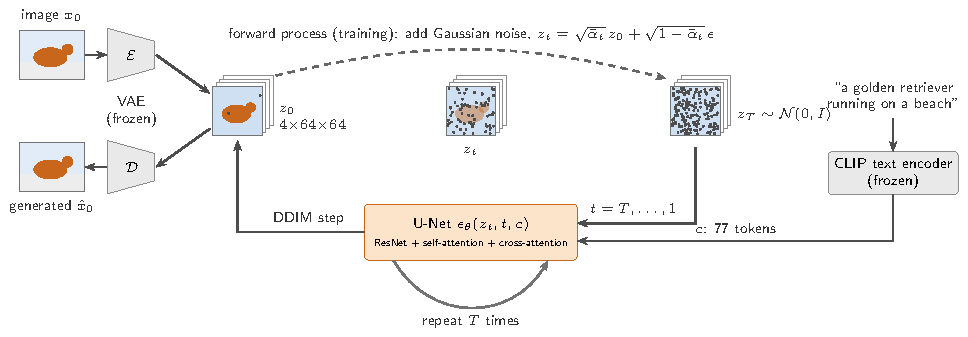
\includegraphics[width=\textwidth]{figures/ldm_pipeline.pdf}
	\caption{Latent diffusion \citep{rombach2022ldm}, the base of AnimateDiff. Training adds noise to
	the VAE latent $z_0$ (Eq.~\eqref{eq:forward}) and trains the U-Net to predict it
	(Eq.~\eqref{eq:eps_loss}). Sampling starts from noise $z_T$ and applies the U-Net, conditioned on
	the CLIP text embedding $c$, for $T$ DDIM steps before the VAE decodes the result.}
	\label{fig:ldm}
\end{figure}

The denoiser $\epsilon_\theta$ is a U-Net \citep{ronneberger2015unet}: an encoder that lowers the
resolution of the latent from $64\times64$ to $8\times8$, a bottleneck, and a decoder that raises it
back, with skip connections between blocks of the same resolution (Figure~\ref{fig:unet}). Each block
has ResNet layers followed by transformer layers built on attention,
\begin{equation}
\mathrm{Attn}(Q,K,V) = \mathrm{softmax}\!\big(QK^\top/\sqrt{d}\big)\,V, \label{eq:attn}
\end{equation}
with the queries $Q$ computed from the image features. In self-attention the keys and values come
from the same features, so every position in the image looks at every other. In cross-attention they
come from the 77 text tokens, which is how the prompt enters the image.

\begin{figure}[!h]
	\centering
	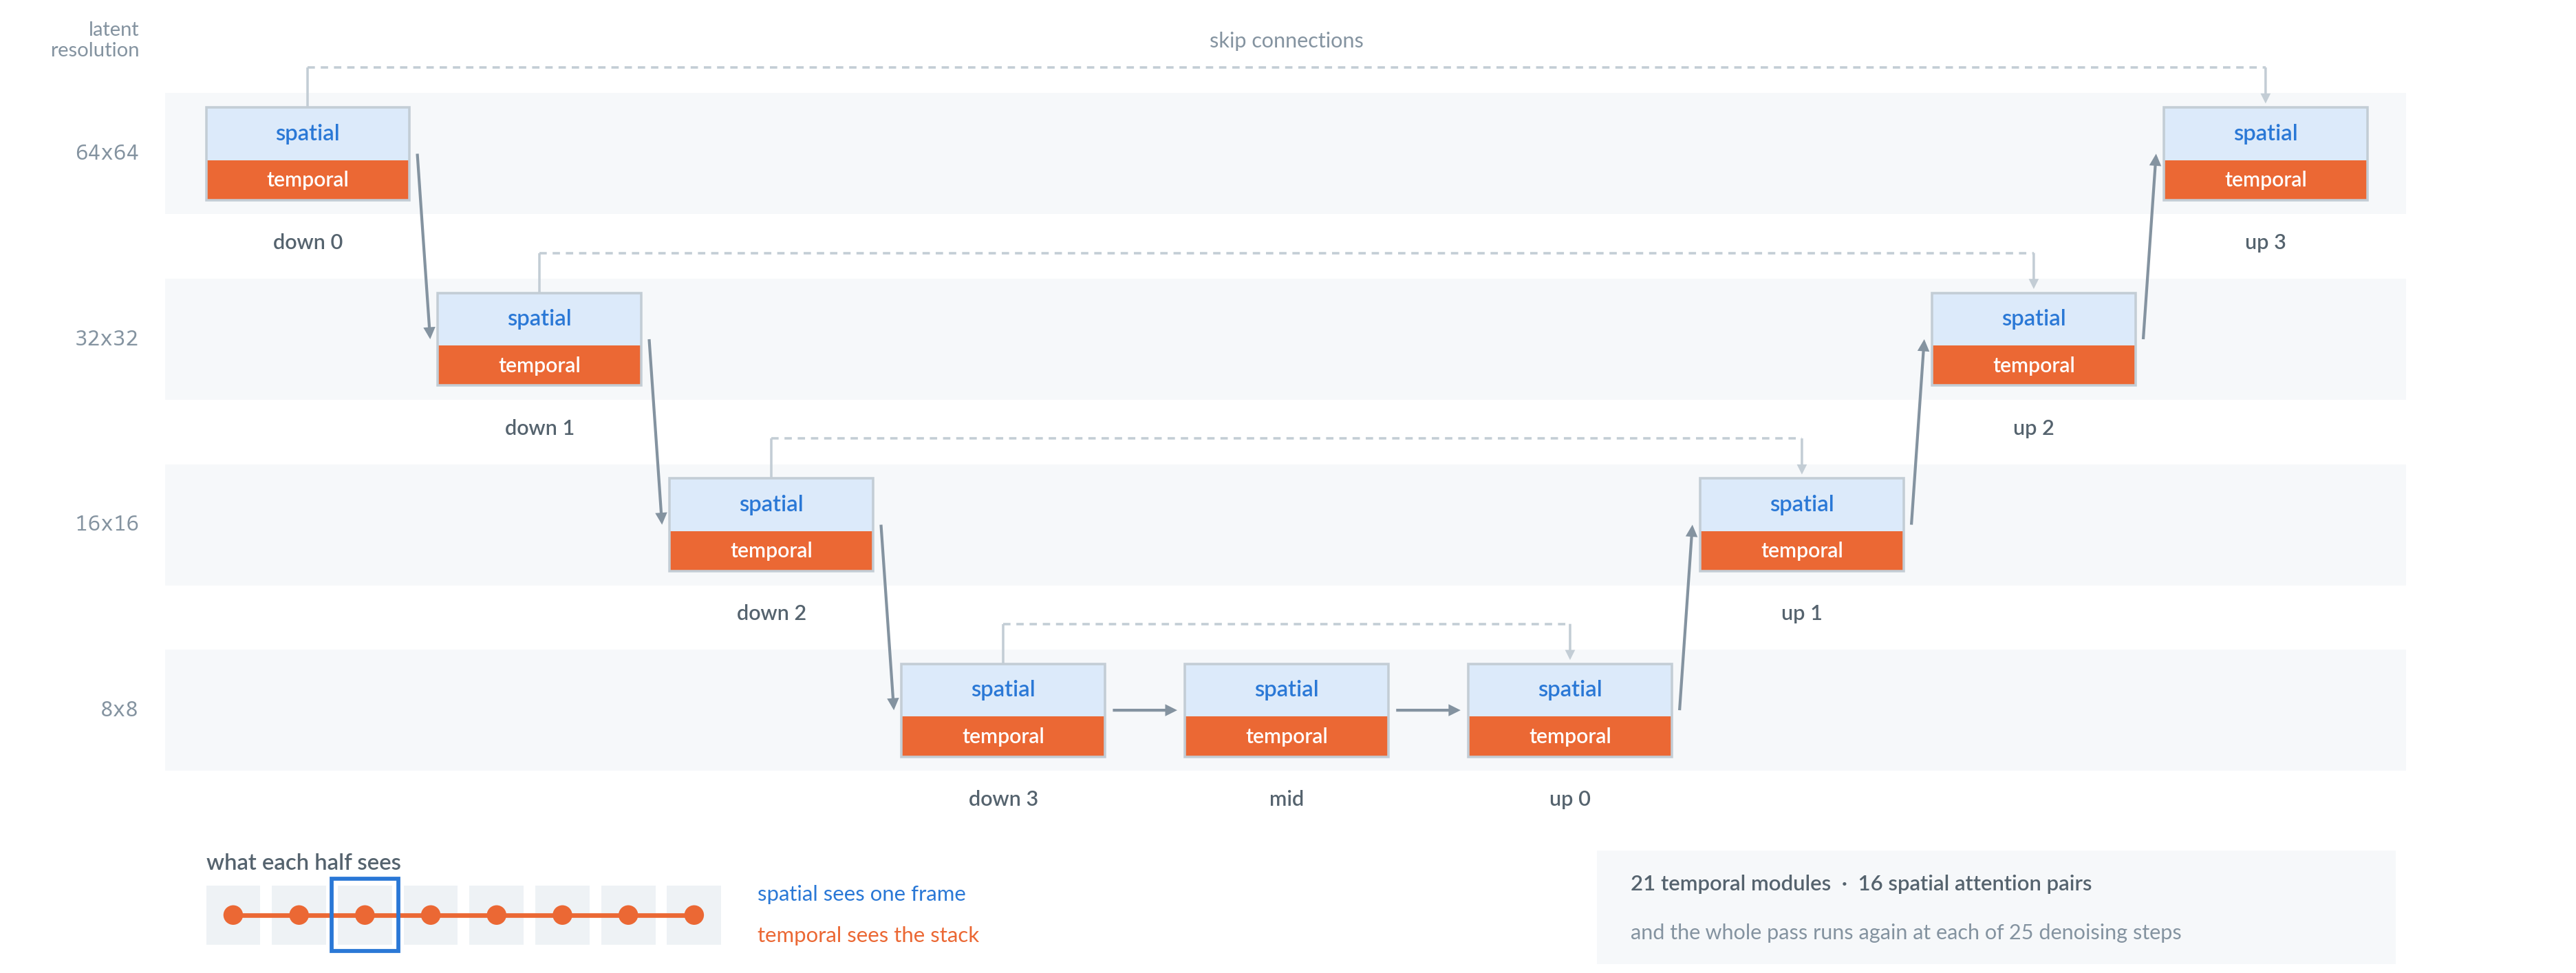
\includegraphics[width=\textwidth]{figures/unet.png}
	\caption{The AnimateDiff U-Net. Each block has a spatial part, which sees one frame, and a temporal
	part, which sees all 16 frames at one position. Skip connections join encoder and decoder blocks of
	the same resolution, and the whole pass runs again at each of the 25 denoising steps.}
	\label{fig:unet}
\end{figure}

A video adds a frame axis. Video Diffusion Models \citep{ho2022vdm} extended the image U-Net by
splitting attention into a spatial part, where the tokens are the positions inside one frame, and a
temporal part, where the tokens are the frames at one position. Video LDM \citep{blattmann2023align}
inserted such temporal layers into a frozen Stable Diffusion and trained only the new layers.
AnimateDiff \citep{guo2024animatediff} takes this furthest. Many fine-tuned copies of Stable
Diffusion~1.5 exist, each drawing a particular style, and the authors train one motion module that can
be attached to any of them without retraining. Training has three stages
(Figure~\ref{fig:animatediff}a): a domain adapter, which is a LoRA \citep{hu2022lora} on the image
layers that absorbs the blur and watermarks of web video and is switched off at inference; the motion
modules, the only weights trained on video; and an optional MotionLoRA that teaches a new camera
motion from 20--50 reference videos. A motion module (Figure~\ref{fig:animatediff}b) reshapes the
activation $x \in \mathbb{R}^{B\times C\times F\times H\times W}$ so that the $F$ frames at each position
form a sequence, applies temporal self-attention (Eq.~\eqref{eq:attn}) with a sinusoidal position
encoding, and adds the result back to its input,
\begin{equation}
z = x + W_{out}\,\mathrm{TempAttn}(x), \qquad W_{out} = 0 \text{ at initialisation}, \label{eq:motion_module}
\end{equation}
so that training starts from the unchanged image model.

\begin{figure}[!h]
	\centering
	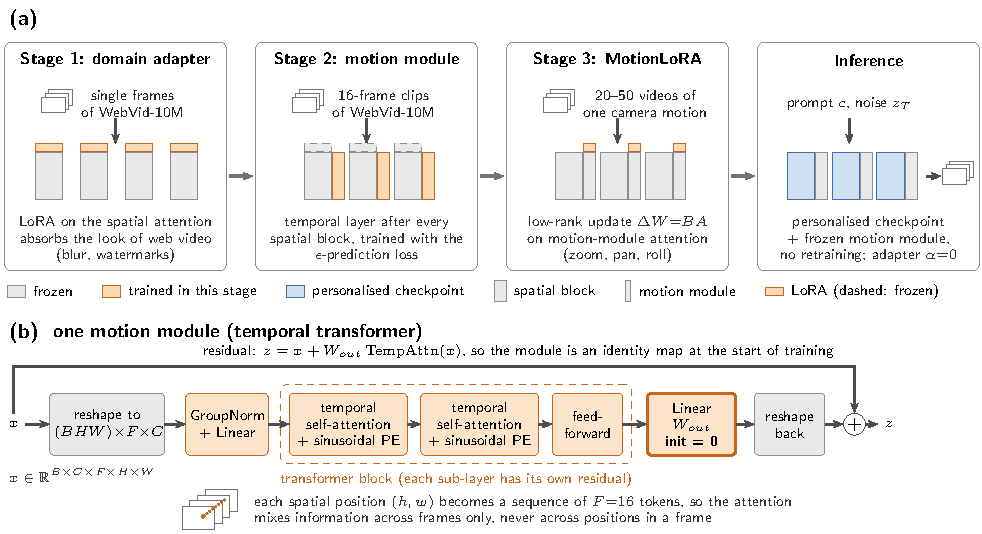
\includegraphics[width=\textwidth]{figures/animatediff_arch.pdf}
	\caption{AnimateDiff \citep{guo2024animatediff}. (a) The three training stages and inference: a
	domain adapter (LoRA on the frozen image U-Net), the motion modules (the only weights trained on
	video), and MotionLoRA. At inference the motion module is attached to a personalised checkpoint.
	(b) One motion module: the activation is reshaped so that the $F$ frames at each spatial position
	form a sequence, passed through temporal self-attention, and added back to its input through a
	zero-initialised output layer.}
	\label{fig:animatediff}
\end{figure}

We chose AnimateDiff because its content and motion weights are physically separate and were trained
at different times. If even this model mixes the two, models trained jointly probably will too. Two
features of the design shape our method. First, because the motion module adds its output to its
input, the activation after it holds content and motion together, so copying it from one generation
into another copies both. Second, because the module already treats the frames as a sequence, it is
natural to split an activation into a part that is the same in every frame and a part that changes
from frame to frame. Knowing which layers are temporal tells us only where motion \emph{could} be
computed, not what those layers hold. For that we needed a way to read motion out of the features,
which MOFT gave us.

Xiao et al.\ \citep{xiao2024moft} found that the features of a video diffusion U-Net mix content and
motion, with most of the channels carrying content. They extract motion in two steps. First they
subtract the mean over the frames, $X - \frac{1}{F}\sum_{i=1}^{F} X_i$, which removes the part that stays
constant over the frames. Then they keep the top 4\% of channels chosen by PCA. The result, called
MOFT, encodes the direction of motion. They read it after a decoder block and use it to guide a new
generation without training, by steering the latents until their MOFT matches a reference. Our
static/dynamic split is their first step, and our layer hypothesis comes from this paper. MOFT shows
where motion can be read from the features, but not whether the model actually uses it there. To
test that, one has to intervene.

The standard tool for intervening in interpretability is activation patching. Meng et al.\
\citep{meng2022rome} introduced it as causal tracing to find where GPT stores facts
(Figure~\ref{fig:patching}a). They run the model on a prompt such as ``The Eiffel Tower is in'',
corrupt the subject's embeddings with Gaussian noise so that the answer is lost, and then restore one
hidden state $h_i^{(\ell)}$ (token $i$, layer $\ell$) to its value from the clean run. The indirect
effect of that state is how much of the answer comes back,
\begin{equation}
\mathrm{IE}\big(h_i^{(\ell)}\big) = P_{*,\,h_i^{(\ell)} \leftarrow \text{clean}}[o] - P_*[o], \label{eq:ie}
\end{equation}
where $P_*[o]$ is the probability of the correct answer $o$ in the corrupted run. Basu et al.\
\citep{basu2024localizing} applied the same procedure to Stable Diffusion, restoring one U-Net layer at
every denoising step. Zhang and Nanda \citep{zhang2024patching} showed that the conclusions depend on
choices that are easy to make carelessly. In particular, Gaussian noise pushes the model off its input
distribution, and they recommend replacing a key token with a related one instead. Heimersheim and
Nanda \citep{heimersheim2024patching} added that the direction matters. Patching from the clean run
into the corrupted one shows whether a state is \emph{sufficient} to restore the behaviour, and the
reverse shows whether it is \emph{necessary} to keep it. The two can disagree when a network has
redundant paths. We follow both papers. Our pairs differ in one word and share the same starting
noise, so neither run is off its distribution. We copy activations at a chosen block over a window of
denoising steps (Figure~\ref{fig:patching}b), and we patch in both directions.

\begin{figure}[!h]
	\centering
	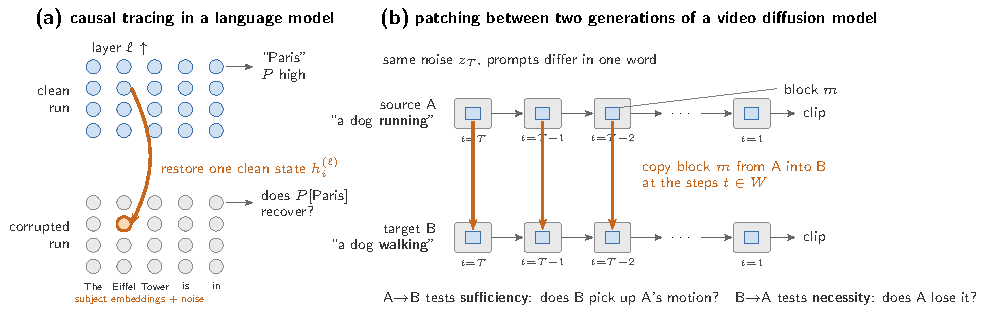
\includegraphics[width=\textwidth]{figures/patching_diagram.pdf}
	\caption{Activation patching. (a) Causal tracing \citep{meng2022rome}: a state from the clean run
	is restored in the corrupted run, and the recovered probability of the answer is its indirect
	effect (Eq.~\eqref{eq:ie}). (b) The same idea for a video diffusion model: two generations from the
	same noise, whose prompts differ in one word, and an activation copied from one into the other at
	block $m$ over a window $W$ of denoising steps.}
	\label{fig:patching}
\end{figure}

Patching a whole activation moves everything a layer carries. The editing literature works more
selectively, inside attention. Image editing methods showed that the attention of Eq.~\eqref{eq:attn}
can be shared between two generations to keep one property while changing another. Prompt-to-Prompt
\citep{hertz2023p2p} reuses the cross-attention maps of one generation in another, so that an edited
prompt keeps the original layout. MasaCtrl \citep{cao2023masactrl} keeps appearance instead: after the
first few steps, the target's spatial self-attention in the decoder queries the keys and values of the
source,
\begin{equation}
\mathrm{Attn}\big(Q_{tgt},\, K_{src},\, V_{src}\big), \label{eq:masactrl}
\end{equation}
so the target takes the source's textures while its own queries keep its own layout. For video,
MotionClone \citep{ling2025motionclone} found that the temporal attention maps of a reference video
carry its motion. It guides the temporal attention of the generated video towards them with
gradients, using a sparse mask that keeps only the strongest link between frames. Diffusion Motion
Transfer \citep{yatim2024dmt} does the same with a loss on space-time features. UniEdit
\citep{bai2024uniedit} combines both operations without any training. It edits motion by injecting
temporal attention from a branch that generates the new motion, and keeps appearance by injecting
spatial self-attention values from a branch that reconstructs the source video. Our attention
injection baseline is the simplest form of these ideas: in each temporal attention layer the target
uses the source's attention probabilities with its own values,
\begin{equation}
\mathrm{softmax}\big(Q_{src}K_{src}^\top/\sqrt{d}\big)\,V_{tgt}. \label{eq:attn_inject}
\end{equation}
We replace the probabilities directly instead of guiding towards them, because a backward pass
through the U-Net at every step was beyond our compute budget. Our later attention-level edits reuse
MasaCtrl's key--value injection for appearance and UniEdit's idea of taking appearance and motion from
two different sources.

Two more works shaped specific choices. Our timestep hypothesis H2 follows the common observation
that diffusion models settle layout and motion in the early denoising steps and appearance later.
Baherwani et al.\ \citep{baherwani2025timesteps} measured this for video diffusion as two regimes with
a fairly consistent boundary between them. Our trained model follows MotionDirector
\citep{zhao2024motiondirector}, which adapts a video model to a reference motion with a dual-path LoRA
\citep{hu2022lora}: one path on the spatial layers for appearance and one on the temporal layers for
motion. We keep only the temporal path and ask whether its placement can come from our maps.

\section{Proposed Approach} \label{sec:our_proj}

Our approach has three steps. First, we generate pairs of clips from the same seed whose prompts
differ in only one word, and record how much the activations at each layer and step respond to that
change. This gives us a map of where content and motion are stored. Second, we intervene on the model
during generation by copying activations or attention from one generation into another at the places
the map points to, and check whether the property we intended to move actually moves. Third, we use
the map for two applications: transferring motion or content between clips, and deciding where to
place small adapters that teach the model a new motion. Apart from the LoRAs and the probes we train
nothing; everything else works on the pretrained model.

Our work differs from existing work in four ways.
\begin{itemize}
  \item Existing editing methods such as MotionClone and MOFT pick the layers to edit either by design
  or by ablation. We first build a map from controlled pairs that measures which layers carry what,
  and then test whether the place where motion is stored is also the place where editing works. In
  our results they are not the same place, and that gap is important to understand.
  \item MOFT uses the frame-mean residual and PCA channels to guide the motion feature at one block.
  We apply the split at every coordinate and step ($S_{dyn}$ vs.\ $S_{stat}$) and then turn it into a
  component patch that moves only one part.
  \item Causal tracing (ROME) and its Stable Diffusion versions study objects in single images. We use
  minimal video pairs and patch in both directions, to see whether a place we found is necessary,
  sufficient, or both for the property we care about.
  \item We place a LoRA where the map says motion is and compare it with a LoRA of similar size placed
  where the map says motion is not. MotionDirector places its LoRA by design.
\end{itemize}

\subsection{Network Architecture}

AnimateDiff is a frozen VAE, a frozen CLIP text encoder and a frozen SD1.5 U-Net, plus motion modules
\citep{hf_animatediff}, sampled with DDIM.
\begin{itemize}
\item \textbf{VAE (frozen, about 84M parameters).} Each 512$\times$512 RGB frame is encoded separately
  into a 4$\times$64$\times$64 latent. Diffusion runs entirely in this latent space, so every activation
  we probe is a function of latents, not pixels.
\item \textbf{CLIP text encoder (frozen, ViT-L/14).} It turns the prompt into 77 tokens of 768
  dimensions each. This is the only way the prompt enters the model, through cross-attention. The same
  embedding is given to all 16 frames, so the text cannot specify motion frame by frame.
\item \textbf{U-Net (frozen, about 860M parameters in the image layers).} This is the denoiser. It has
  4 encoder blocks that lower the resolution from 64$\times$64 to 8$\times$8 while the channels grow from
  320 to 1280, a middle block, and 4 decoder blocks that raise the resolution back to 64$\times$64. Skip
  connections pass encoder features to the decoder. Layout and trajectory are visible at low
  resolution, appearance and texture at high resolution. The skip connections are also why the
  outermost decoder block can be a strong patch site: it combines encoder detail with the decoded result.
\item \textbf{ResNet layers and timestep embedding.} Each ResNet layer applies GroupNorm, SiLU and
  3$\times$3 convolutions to each frame, with a residual connection. The denoising step enters as a
  sinusoidal embedding passed through an MLP and added to the features after the first convolution.
  This is why one layer can do different jobs at different steps, and why our map has to cover steps
  as well as layers.
\item \textbf{Spatial transformer.} Each one has a self-attention layer, where every position attends
  to the others in the same frame, a cross-attention layer, where image positions attend to the text
  tokens, and a feed-forward layer, all with residual connections. Frames are batched, so these layers
  cannot see other frames. Self-attention keeps appearance consistent within a frame and is what
  appearance-transfer methods use. Cross-attention is where we hook our content coordinates and where
  the subject masks (DAAM) come from.
\item \textbf{Motion modules (21 modules, about 417M parameters).} One is inserted after the spatial
  layers in each block. It reshapes the activation from $(B\cdot F, C, H, W)$ to $(B\cdot H\cdot W, F, C)$
  so that the frames form a sequence, adds a sinusoidal position embedding, applies two temporal
  self-attention layers and a feed-forward layer, and adds the result back to the input through a
  zero-initialised output layer (Eq.~\eqref{eq:motion_module}). Temporal attention is the only place
  where information crosses between frames, so it is the only place where motion can be computed.
  Without the position embedding, forward and backward motion would look the same. The residual
  addition is why content and motion mix in the module's output, so we cannot simply copy the whole
  output of a layer. The attention probabilities are frame-to-frame matrices, and they are what our
  attention injection baseline copies.
\item \textbf{DDIM sampler.} The deterministic sampler means that the same seed always gives the same
  clip, which our controlled pairs and patching rely on. Under classifier-free guidance (scale 7.5)
  every U-Net call processes an unconditional and a conditional copy, and our patches act on both by
  default.
\end{itemize}

This architecture suits us because its layers are clearly separated, so each one can be hooked and
patched. It is text-conditioned, so we can build controlled pairs. And its image weights were frozen
while the motion modules were trained, which should make the two easier to separate. The cost is that
some of the separation is built in by the training recipe, so we also need to probe other models.

\subsection{Work done before the prep-presentation review} \label{sec:before}

\textbf{Choice of model.} We compared three open models. AnimateDiff has an explicit spatial/temporal
split in its module tree, good diffusers support, and fits on a T4 (10.2\,GB measured). ModelScope T2V
(1.7\,B parameters) trains space and time together, which makes it the harder and more interesting
case, but the tools for extracting its attention are less mature. Stable Video Diffusion has the best
output quality but is conditioned only on an image, so we could not build pairs from one-word prompt
changes. We chose AnimateDiff for all deliverables and kept ModelScope as a later robustness check.

\textbf{Definitions and protocol.} Following the brief, content is what an image classifier would see
in a single frame (subject identity, colour, texture, layout), and motion is how pixels move across
frames, regardless of what they belong to. To separate the two inside the network we split every
activation $x$ with $F$ frames into its frame mean and the residual around it,
\begin{equation}
x_f = \xs + \xd_f, \qquad \xs = \frac{1}{F}\sum_{f=1}^{F} x_f, \qquad \xd_f = x_f - \xs. \label{eq:split}
\end{equation}
The static part $\xs$ is the same in every frame, and the dynamic part $\xd$ is everything that
changes from frame to frame. We kept a register of decisions (\code{code/docs/protocol.md}), 22 of which
were fixed before the review: among them the distance ($1-\cos$), the split above, how pairs are
formed, the edit metric, the success criterion and the baseline.

\textbf{Three hypotheses with fixed tests.} Each one makes a prediction that could fail.
\begin{itemize}
\item \textbf{H1 (layer).} Motion selectivity peaks in a medium-resolution decoder block
  (\code{up_blocks.1}), following MOFT \citep{xiao2024moft}. Test: the bootstrap argmax over the nine
  temporal blocks of $M(b) = -\mathrm{mean}_t\,\mathrm{median}\,S_{dyn}(b,t)$ must exclude the
  extreme-resolution blocks. ($S$ is defined in Section~\ref{sec:after}.)
\item \textbf{H2 (timestep).} Motion is settled early in denoising. Test: a single least-squares
  changepoint $\tau$ on the winning block's profile must fall in the first half, with the early
  segment above the late one.
\item \textbf{H3 (representation).} The frame mean $\xs$ is dominated by content, and removing it
  reveals motion selectivity that the raw activation hides. Test: at least 75\% of coordinate-steps
  have $S_{stat}$ significantly content-selective, and at least one temporal coordinate flips from
  content-selective in $\xs$ to motion-selective in $\xd$.
\end{itemize}

\textbf{Pilots E1--E3 (Kaggle T4).}
\begin{itemize}
\item \textbf{E1, cost.} 94.1\,s and 10.2\,GB per clip on a T4 at our settings, so the full 360-clip
  probing set needs about 9.4 GPU-hours.
\item \textbf{E2, does a fixed noise tensor isolate a word?} We generated seven clips from one noise
  tensor: ``a golden retriever running on a beach'', three subject swaps and three verb swaps. Subject
  swaps moved CLIP appearance 2.6$\times$ more than verb swaps, so the content side of the control works.
  The motion side failed. A frame-difference motion measure moved \emph{more} under subject swaps (0.461)
  than under verb swaps (0.390), because frame differences sit on the outline of the object, and a new
  object has a new outline (Figure~\ref{fig:e2}). Pixel motion is mixed up with content. This is why we
  measure selectivity on the residual $\xd$, and why content pairs only swap subjects within a body-plan
  family (a dog for a wolf, not a dog for a person).
\item \textbf{E3, can we get the activations out?} Hooks on all 95 modules cost 0.6\% of generation
  time if they only record metadata. A full fp16 dump of every coordinate at every step is 87.9\,GiB per
  clip, while a summary (channel statistics, per-frame residual norms, one 16$\times$16 map per attention
  layer) is 44.6\,MiB, 2{,}017$\times$ smaller. Storing full activations for 360 clips was impossible,
  which forced us to score pairs during generation (Section~\ref{sec:after}).
\end{itemize}

\begin{figure}[!h]
	\centering
	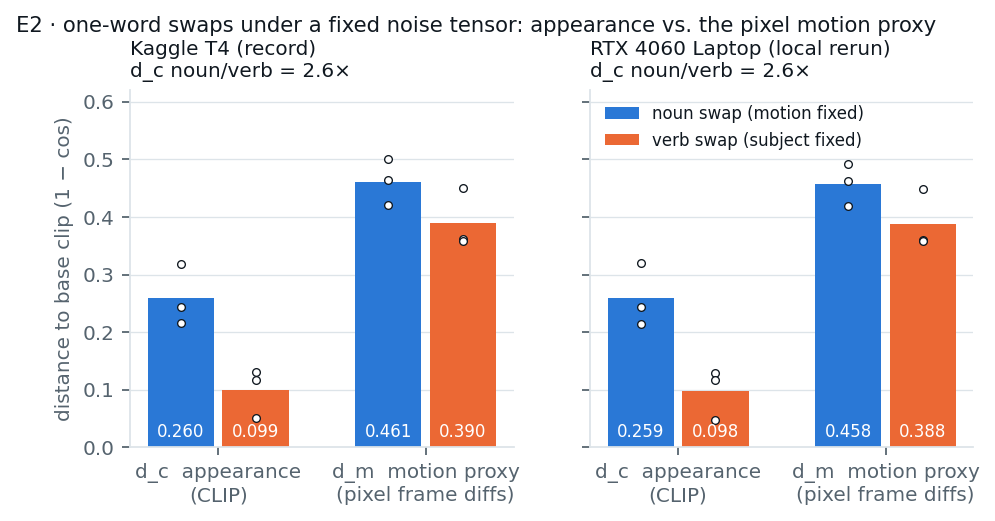
\includegraphics[width=0.82\textwidth]{figures/e2_pixel_confound.png}
	\caption{Pilot E2. A pixel-space motion measure changes more when the subject is swapped (motion
	held fixed) than when the verb is swapped. Measuring motion in pixel space would have mistaken
	content for motion.}
	\label{fig:e2}
\end{figure}

\subsection{Work done after the prep-presentation review} \label{sec:after}

Several things changed after the review. The pilots showed that storing activations was impossible,
which led to the lockstep sampler and online scoring. The probing sweep then falsified H1 and H3, so
the map did not give us a clean motion layer to patch. The component patches chosen from the map did
not meet our criterion on the test pairs either. This sent us back to the literature for
attention-level operators, and to H2's timing, which we could use directly by switching the prompt.
Finally, we repeated the probing on three more model variants and added causal tests in both
directions, to check whether the map is specific to one model.

\textbf{Lockstep sampler and online scoring.} A selectivity map needs, for every pair, the distance
between two clips' activations at every coordinate and step. Caching one clip's activations at all 25
steps for 16 coordinates takes about 7.6\,GB of host memory, and a group has 21 such anchor clips. We
instead denoise all 60 clips of a (seed, scene) group \emph{in lockstep}. At step $t$ every anchor runs
and its step-$t$ activations are kept, then every partner runs and is scored against them, and then the
step-$t$ activations are dropped. Memory holds one step instead of 25, every clip is generated exactly
once, and distances are computed on the full tensors rather than on summaries. The loop re-implements
diffusers' \code{AnimateDiffPipeline} step by step. Before using it we checked on the GPU that a clip
generated alone, inside a group, and with all probes attached gives a final latent identical to
\code{pipe()} (mean absolute difference exactly 0).

\textbf{Selectivity.} For one coordinate $(L,t)$, let $d_c$ be the distance across a content pair
(subject swapped) and $d_m$ across a motion pair (verb swapped). Then
\begin{equation}
S = \frac{d_c - d_m}{d_c + d_m} \in [-1, 1], \label{eq:sel}
\end{equation}
which is positive when the coordinate tracks what is shown and negative when it tracks how things
move. $S_{dyn}$ uses $\xd$ and $S_{stat}$ uses $\xs$. Since $d_c$ and $d_m$ come from different pairs, we
compute $S$ on matched units. A unit is a clip $B$ = (subject $s$, verb $v$, scene) that is the end point
of both a content pair, (family anchor, $v$) $\to B$, and a motion pair, ($s$, running) $\to B$. This gives
78 units per seed. Each map cell is the median over units, with a 1{,}000-sample bootstrap CI within each
seed, averaged over the three seeds.

\textbf{Linear probes.} To check whether motion information is \emph{present} even where selectivity is
low, we trained logistic-regression probes for the verb (4 classes) and the subject's family (2 classes)
at each coordinate and step. Since we could not store full tensors, each clip's $\xd$ and $\xs$ were
compressed with a count sketch to 512 dimensions, a random projection that preserves inner products in
expectation. The pipeline is standardisation, PCA fitted on the training split only, and logistic
regression ($C=1$). We trained on one scene and tested on the other, so a probe cannot succeed by
memorising the background.

\textbf{Component patching.} A patch replaces part of the target generation's activation at a
coordinate with the source generation's. Besides the usual whole-tensor, channel-subset and
$\alpha$-scaled patches, we added a \emph{component} patch that moves only one term of
Eq.~\eqref{eq:split}:
\begin{align}
\text{dynamic:}\quad & x_{out} \leftarrow \xs_{tgt} + \xd_{src}, &
\text{static:}\quad & x_{out} \leftarrow \xs_{src} + \xd_{tgt}.
\end{align}
The motion modules write into the residual stream, so a whole-tensor patch there copies content and
motion together. The split that defines the map is the natural way to move one and keep the other.
In fp16 the obvious implementation is not exact: patching a clip with itself drifted to a mean absolute
difference of $10^{-2}$ over 25 steps. We therefore compute the dynamic patch as
$x_{out} + (\delta - \bar\delta)$ with $\delta = x_{src} - x_{out}$, which is exactly zero for a self-patch.
Algorithm~\ref{alg:edit} shows one edit.

\begin{algorithm}[!h]
\caption{One edit: source A and $N$ target arms denoised in lockstep from one noise tensor}
\label{alg:edit}
\begin{algorithmic}[1]
\Require noise $z_T$, prompts $p_A$ (source) and $p_{tgt}$, arms $\{(\text{coords}_k, \text{steps}_k, \text{component}_k, \alpha_k)\}_{k=1}^N$
\State $z^{A} \gets z_T$; \; $z^{k} \gets z_T$ for $k = 1..N$
\For{$t$ in the 25 DDIM steps}
  \State run U-Net on $z^{A}$ with $p_A$; cache A's outputs at every coordinate any arm patches at $t$
  \For{$k = 1..N$}
    \State run U-Net on $z^{k}$ with $p_{tgt}$; at each $c \in \text{coords}_k$, if $t \in \text{steps}_k$:
    \State \hspace{1em} $\delta \gets x^A_c - x^k_c$; \; $x^k_c \gets x^k_c + \alpha_k \cdot \mathrm{part}(\delta)$
      \Comment{part $=\delta-\bar\delta$ (dynamic), $\bar\delta$ (static) or $\delta$ (whole)}
    \State $z^{k} \gets \mathrm{DDIM}(z^{k}, \hat\epsilon^{k}, t)$
  \EndFor
  \State $z^{A} \gets \mathrm{DDIM}(z^{A}, \hat\epsilon^{A}, t)$; free the step-$t$ cache
\EndFor
\end{algorithmic}
\end{algorithm}

\textbf{Temporal attention injection (baseline).} In each temporal attention layer the target uses the
source's attention probabilities $P_{src}$ instead of its own over a chosen window of steps, with its own
values $V$ (Eq.~\eqref{eq:attn_inject}). For the same fp16 reason we compute it as
$\mathrm{SDPA}(Q,K,V) + \alpha\, W_{out}\big((P_{src}-P)V\big)$, which equals
$\big((1-\alpha)P + \alpha P_{src}\big)V$ in exact arithmetic and is exactly null when a clip is injected
into itself.

\textbf{Edit directions and the metric $D$.} Clips A and B differ in both subject and verb. In the
\emph{motion} direction the target prompt is B's subject with A's verb and we patch $\xd$, so the output
should look like B and move like A. In the \emph{content} direction the target prompt is A's subject with
B's verb and we patch $\xs$. We score content fidelity $s_c$ as the mean per-frame CLIP image cosine
\citep{radford2021clip}, and motion fidelity $s_m$ as the cosine between dense Farneb\"ack optical-flow
fields \citep{farneback2003}, averaged over frame pairs. For the motion direction
\begin{equation}
D = \tfrac12\big[\hat s_c(\text{out},B) + \hat s_m(\text{out},A)\big] - \tfrac12\big[\hat s_c(\text{out},A) + \hat s_m(\text{out},B)\big], \label{eq:D}
\end{equation}
with A and B exchanged for the content direction, and $\hat s$ min-max normalised over all values in one
scoring run (the ``pool''). $D$ rewards taking the right property from each clip and penalises taking
the wrong one. The number we report is $\dD = D(\text{arm}) - D(\text{prompt only})$ on the same pair,
which is what the edit adds over simply changing the prompt. Our pre-registered success criterion has
three parts: in both directions, the median $\dD$ is positive, its 95\% paired-bootstrap CI over pairs
excludes zero, and subject consistency stays within 10\% of the source clip's.

\textbf{Attention-level edits.} The component patches write into the residual stream, and that stream
carries both content and motion. H3 had already shown that even the frame mean $\xs$ of a motion module
carries some motion, so a static patch also drags some motion along. The editing methods in the
literature work one level lower, inside attention. They only change what each position looks at, and
the target keeps its own queries, so it keeps its own layout. We built three such operators and tested
them with the same pairs, metric and criterion as before. The operators and the rule for picking one
were written down before any of them ran. Since the test pairs had already been used once, we treat this
stage as exploratory and report it separately from the pre-registered result.
\begin{itemize}
\item \textbf{Key/value injection} into spatial self-attention, following MasaCtrl \citep{cao2023masactrl}
  and the content branch of UniEdit \citep{bai2024uniedit}. From a chosen step onwards, the target's
  spatial self-attention uses its own queries with the source's keys and values
  (Eq.~\eqref{eq:masactrl}). The target gets the source's appearance but keeps its own layout and
  motion. In the frame-wise version frame $f$ reads source frame $f$. In the frame-0 version every frame
  reads source frame 0, because frame-wise keys and values also carry each source frame's layout, and
  with it some of the source's motion.
\item \textbf{Temporal attention injection over all 25 steps}, the motion branch of UniEdit. This is
  the baseline operator (Eq.~\eqref{eq:attn_inject}) applied over the whole trajectory instead of the
  first third.
\item \textbf{Dual-source edits}, where appearance comes from one clip and motion from the other. In the
  motion direction the output takes A's temporal attention and B's spatial keys and values. In the
  content direction it takes A's keys and values and B's temporal attention.
\end{itemize}
For placement we first used what the papers use: keys and values in \code{up_blocks.2}--\code{3} or in
every decoder block, starting from step 2 or step 5, and temporal attention in all modules, in
\code{up_blocks.0}, or in \code{up_blocks.1}, the block that MotionClone \citep{ling2025motionclone} and
MOFT \citep{xiao2024moft} use. We then added three \emph{probe-placed} arms whose placement comes from
our own map: temporal attention in \code{up_blocks.0} and the mid block (the blocks that lean towards
motion under H1), at steps 0--2 (the H2 window) and at all steps, and keys and values in
\code{down_blocks.2}, which has the strongest content selectivity in $S_{stat}$. That makes 7 motion and
7 content arms, run on the 4 dev pairs. The rule picks, for each direction and each family (single- or
dual-source), the arm with the highest median $\dD$ among the arms whose subject-consistency ratio is at
least 0.9, with ties going to fewer modules. It picked:
\begin{itemize}
\item motion, single: temporal attention in every module at every step;
\item motion, dual: the same, plus B's keys and values in \code{up_blocks.2}--\code{3} from step 2;
\item content, single: the probe-placed keys and values in \code{down_blocks.2};
\item content, dual: A's keys and values with B's temporal attention at every step.
\end{itemize}
As with the patches, injecting a clip's own keys and values into itself gives back exactly the same clip.

One thing has to be said about the dual-source arms. They read clip B and are then scored partly
against B ($s_c(\text{out},B)$ in the motion direction, $s_m(\text{out},B)$ in the content direction), so
part of their score comes from the way they are built. They answer a different question: whether we can
swap motion and appearance between two clips, not whether we can edit a clip with a new prompt. So we
report them as a separate family and do not compare them with the prompt-only edit as if they were the
same kind of edit.

\textbf{Prompt switching timed by H2.} H2 says that motion is decided in the first two of the 25 steps.
If that is true, an edit should not need any surgery inside the network. We can denoise with one prompt
for the first $\tau$ steps and then switch to the other. In the motion direction we start with A's
prompt and switch to (B's subject, A's verb) at step $\tau$. In the content direction we start with (A's
subject, B's verb) and switch to A's prompt. Every track starts from the pair's shared noise. We also
built a \emph{masked} switch for the motion direction, following EIDT-V \citep{jagpal2025eidtv}. From step
$\tau$ on, the latent becomes $z \leftarrow M\cdot z + (1-M)\cdot z_A$, where $M$ is A's subject mask, so
everything outside the subject stays as it is in A. The mask comes from A's cross-attention, aggregated
as in DAAM \citep{tang2023daam} but keeping the frame axis: the attention on the subject's tokens is
averaged over heads, upsampled, summed over the 16 spatial cross-attention layers and all 25 steps,
thresholded at 0.4 of each frame's maximum and dilated by 7 latent pixels. The pre-registered arms use
$\tau = 2$, the H2 changepoint. That number came from the probing sweep, so nothing was chosen on the edit
pairs. The other values ($\tau \in \{1, 3, 5, 8\}$, and masked $\tau = 3$) are exploratory and show how
the result changes with the switch time. If the H2 timing is causal, the curve should bend sharply near
$\tau = 2$. So this stage is both a test of H2 and an editing method.

\textbf{Motion LoRAs (the trained model).} LoRA \citep{hu2022lora} adds a trainable low-rank update
$\Delta W = \frac{\alpha}{r}BA$ to frozen weight matrices. We put LoRA on the query, key, value and output
projections of the temporal attention layers, in three placements with the same rank, data and number
of steps:
\begin{itemize}
\item \code{full}: all 21 motion modules (9.67\,M trainable parameters);
\item \code{probe}: only \code{up_blocks.0}, the block chosen by the H1 bootstrap (1.97\,M);
\item \code{anti}: \code{down_blocks.2} and \code{.3}, the two blocks with the lowest $M(b)$ (2.62\,M),
  as a wrong-place control.
\end{itemize}
Without the control, ``\code{probe} is as good as \code{full}'' could mean that any block would do. The
\code{anti} LoRA is a bit bigger than \code{probe}, so if \code{probe} wins it cannot be because it has
more parameters. The loss is the model's own $\epsilon$-prediction objective (Eq.~\eqref{eq:eps_loss}),
\begin{equation}
\mathcal{L} = \mathbb{E}_{z_0, \epsilon, t}\,\big\| \epsilon - \epsilon_\theta(\sqrt{\bar\alpha_t}\,z_0 + \sqrt{1-\bar\alpha_t}\,\epsilon,\ t,\ c) \big\|_2^2,
\end{equation}
on 16-frame VAE latents $z_0$ of real clips with caption $c$ = ``a person \{verb\}'', and only the LoRA
matrices receive gradients. We chose LoRA over fine-tuning the whole motion adapter because it trains
about 2--10\,M parameters instead of 417\,M, so it fits on our 8\,GB laptop GPU, and we can control
exactly where it goes. We put it only on the temporal attention projections because that is where
information moves across frames, which is also the choice in the temporal path of MotionDirector
\citep{zhao2024motiondirector}.

\textbf{Upload path: DDIM inversion.} Every edit needs a source track whose activations we can cache at
every step. An uploaded video has no generation behind it, so we make one. The video is cut to its
longest shot (a cut is a jump in mean grey-level difference between frames larger than both 4$\times$
the clip's median jump and 20), resampled to 16 frames, encoded with the VAE and inverted with
deterministic DDIM (text-conditional only, no guidance) onto the same 25 timesteps the sampler uses. Each
inversion step goes from a cleaner latent $z_k$ to a noisier one,
\begin{equation}
\hat z_0 = \frac{z_k - \sqrt{1-\bar\alpha_k}\,\epsilon}{\sqrt{\bar\alpha_k}}, \qquad
z_{k+1} = \sqrt{\bar\alpha_{k+1}}\,\hat z_0 + \sqrt{1-\bar\alpha_{k+1}}\,\epsilon,
\end{equation}
with $\epsilon$ predicted at $z_k$. During the edit the source track follows this trajectory: at each step
the U-Net sees the inverted latent, so the cached activations are the video's. The new clip does not
start from the inverted noise itself, because inverted latents are not Gaussian, and sampling from them
with guidance 7.5 gives blotchy, grid-patterned clips even without any edit. Instead it starts from the
inverted noise and the seed's Gaussian noise added with equal weight and rescaled to unit variance.
Section~\ref{sec:res_upload} compares this start with the other two.

\textbf{Experiment 2: other models and causal tests.} Experiment 1 had three weak points. First, motion
was just a word. Our only motion label was the verb in the prompt, and the frozen SD1.5 base changes
appearance a little from frame to frame, so $\xd$ holds appearance drift as well as real movement. Every
layer after cross-attention also sees the verb token, so a verb probe can succeed without any motion
being represented. Second, our grid was coarse. We probed one motion module per block, while
\code{up_blocks.1}, the motion site in MOFT, MotionClone and DMT \citep{yatim2024dmt}, has three. Third,
our causal tests went in one direction only and used 12 pairs. Patching in one direction tests whether
a site is sufficient but not whether it is necessary \citep{heimersheim2024patching}, and from the width
of our CIs we would need about 25 pairs per claim to detect an effect of 0.10. Experiment 2 was built to
fix each of these, and all its rules were fixed before any of its data were generated.

\emph{Four models.} We crossed the image weights, SD1.5 or epiCRealism \citep{hf_epicrealism} (a
community fine-tune of SD1.5), with the motion weights, adapter \mbox{v1-5-2} \citep{hf_animatediff} or
\mbox{v1-5-3} \citep{hf_animatediff_v3}. Only these weights change. The sampler, prompts and noise are the
same in all four cells, so every comparison between cells is paired by prompt and noise. Swapping the
base tells us whether the motion site depends on the image features that go into the motion modules,
and swapping the adapter tells us whether it belongs to the motion prior. The \mbox{v1-5-3} adapter has no
motion module in the mid block (20 instead of 21), so we match coordinates by block and position. Each
cell has 240 clips: the probing vocabulary with seeds 42 and 1337 and both scenes. Seed 2024 was kept
aside for the causal tests.

\emph{A finer sweep and measured motion.} The sweep hooks 117 coordinates: the 95 from Experiment 1 plus
22 ResNet outputs, because Basu et al.\ \citep{basu2024localizing} found that much of Stable Diffusion's
knowledge sits in the ResNets and self-attention rather than in cross-attention. Every coordinate is
count-sketched to 512 dimensions, and $\xd$ in the \code{up_blocks.0} and \code{up_blocks.1} coordinates is
sketched to 2{,}048 dimensions at steps 0--14, since sketched cosines close to zero are noisy at 512.
Distances between pairs are still exact and computed online in lockstep. To turn motion into something
we measure, we ran RAFT optical flow \citep{teed2020raft} on every clip, removed camera motion by
subtracting the median background flow, and used the DAAM subject masks to keep only the subject's flow.
CLIP frame embeddings are the content measure.

\emph{Quality gate.} Before choosing one cell for the expensive steps we scored all 960 clips with checks
from VBench \citep{huang2024vbench}: subject consistency (DINO \citep{caron2021dino} similarity of each
frame to the first and to the previous frame), dynamic degree (a clip moves if enough frame pairs have a
large top-5\% RAFT flow), CLIP-T for text alignment, and X-CLIP \citep{ni2022xclip} to check that the verb
is recognisable. The rule was to take the highest subject consistency among the cells with a dynamic
share of at least 0.5 and CLIP-T within 0.01 of the best. No cell passed both conditions. Both epiCRealism
cells hardly move (dynamic share 0.021 and 0.004), and both SD1.5 cells missed the CLIP-T tolerance by
0.001--0.002. The rule did not cover this case, so before anything else ran we dropped the CLIP-T
condition and kept the motion one, because subject consistency on its own rewards videos that do not
move. The primary cell is SD1.5 with \mbox{v1-5-2}, the same model as Experiment 1.

\emph{Looking for presence.} On each cell we ran the following.
\begin{itemize}
\item \textbf{A confirmatory test} of Experiment 1's motion site (\code{up_blocks.0} motion module 2,
  steps 0--2, $S_{dyn}$). We take each subject's mean selectivity and run an exact one-sided sign-flip test
  over the 13 subjects that appear as the end point of a matched unit ($2^{13}$ sign patterns). The site
  replicates if $p < 0.05$. This is the only confirmatory test, and everything else in this list is
  exploratory.
\item \textbf{Selectivity maps} with a sign-flip $t$ in every cell and max-$|t|$ family-wise correction
  over the whole map.
\item \textbf{ANOVA variance fractions.} The design is balanced, so the variance of an activation splits
  exactly into subject, verb, scene, seed, subject$\times$verb and residual fractions. This gives a direct
  ``how much is content and how much is motion'' number for each layer.
\item \textbf{RSA with variance partitioning} \citep{kriegeskorte2008rsa}. For each layer and step, the
  clip-by-clip distance matrix is regressed on three model matrices: content (CLIP image embeddings),
  motion (subject-masked flow) and the prompt's CLIP text embedding. The \emph{unique} motion share is
  the part that flow explains beyond content and text. Significance comes from permuting clips within a
  seed (49 draws) with max-over-map correction.
\item \textbf{Debiased CKA} \citep{kornblith2019cka} to compare layers across cells. With 60--120 clips and
  512 features ordinary CKA is high even for random matrices, so we use the unbiased version.
\item \textbf{Flow decoding gain.} Ridge regression decodes the part of the flow that changes
  \emph{within} a prompt (across seeds) from the layer's $\xd$, and separately from the step-$t$ latent.
  The gain $G = \max(R^2_{layer},0) - \max(R^2_{latent},0)$ is the motion information the layer adds over
  the noisy latent. Variation within a prompt is the one kind of motion that the prompt itself cannot
  explain.
\item \textbf{Channel selectivity}, in the style of MOFT, to see whether motion sits in a few channels.
\end{itemize}
After analysing the first cell, and before selecting anything, we found and corrected three mistakes in
the analysis. The ridge strength had been chosen by leave-one-clip-out CV, which leaks through the paired
residuals of a prompt's two seeds, so we replaced it with grouped 4-fold CV over subjects. The RSA was
missing the text-embedding matrix that the design asked for; without it the motion share came out
significant in 82\% of cells, partly because the verb word reaches every layer through the text. And
channel energies stored in fp16 underflowed, so we recomputed them in fp64.

\emph{Testing use.} The pre-registered rule picked four candidate sites on the primary cell:
(1) Experiment 1's site, \code{up_blocks.0} motion module 2 at steps 0--2, on $\xd$; (2) the coordinate
with the highest unique RSA motion share, in a five-step window around its peak, on $\xd$; (3) all three
\code{up_blocks.1} motion modules at steps 0--7, on $\xd$, the site from the literature; and (4) the
coordinate with the highest unique RSA content share, around its peak, on $\xs$. Each was tested on 25
motion and 25 content pairs drawn from the held-out seed 2024, by patching in three ways:
\begin{itemize}
\item A$\to$B, running B with A's activation, which tests whether the site is \emph{sufficient};
\item B$\to$A, running A with B's activation, which tests whether it is \emph{necessary};
\item C$\to$B, patching from an unrelated clip C, which separates ``carries A's property'' from ``any
  disruption at all''.
\end{itemize}
Following Zhang and Nanda \citep{zhang2024patching} we normalise the effect,
\begin{equation}
\mathrm{PE}_P = \frac{D_P(x_{patch}) - D_P(x_B)}{D_P(x_A) - D_P(x_B)},
\end{equation}
where $D_P$ is a contrastive score for property $P$ (for motion, flow similarity to A minus flow
similarity to B). PE is 0 when nothing transfers and 1 when everything does. The necessity effect NE is
defined in the same way for B$\to$A. The CIs come from a bootstrap over subjects.

As a second test of necessity we used LEACE \citep{belrose2023leace}, a closed-form eraser that makes a
concept linearly unpredictable while changing the activation as little as possible. We fitted it on a
candidate's $\xd$ with the verb as the concept (rank at most 3) and applied it as a hook during sampling.
The control is a random erasure of the same rank, as in amnesic probing \citep{elazar2021amnesic}: if
LEACE hurts the motion more than the random erasure does, the directions it removed were being used. We
re-centred the eraser over frames so that it does not shift $\xs$.

To put all of this together we wrote a decision rule, combining ideas from Hewitt and Liang
\citep{hewitt2019control}, amnesic probing and Heimersheim and Nanda. The combination is our own.
\begin{itemize}
\item \textbf{E, presence:} the site's unique RSA share, or its decoding gain, is significantly above zero.
\item \textbf{S, sufficiency:} the CI of its A$\to$B effect is above zero and above the C$\to$B control.
\item \textbf{N, necessity:} the CI of its B$\to$A effect is above zero, or LEACE hurts more than random
  erasure.
\item \textbf{D, dissociation:} the site moves its own property while the other property stays within
  $\pm 0.1$.
\end{itemize}
A site ``encodes but does not use'' a property when E holds and both S and N fail. It ``uses'' the
property when S or N holds, and we say which one. We would only call a site \emph{the} motion site if it
showed a double dissociation against a content site.

\emph{Content ladder and parts not run.} To turn one-word swaps into dose-response curves, the ladder
changes the subject in steps: a null step (``a dog'' $\to$ ``one dog''), then colour, coat, breed, species,
scene and lighting, for 8 base animals $\times$ 2 verbs (walking and running, the two that X-CLIP
recognised best) $\times$ 7 variants $\times$ 2 seeds. Each layer's distance is regressed on the measured
CLIP content change and the measured flow change, which gives the layer's sensitivity to content with
the motion taken out. This run was still going when we wrote this report. The design also had a LoRA
test (modules picked by the probes against 19 random module sets with the same number of parameters,
scored with the Motion Fidelity Score of DMT), MDL probing \citep{voita2020mdl} and attribution patching.
We could not run these within our compute budget.

\textbf{Interface.} The brief asks for an interface where a user can test the method on their own
inputs. We built a Gradio app (\code{scripts/app.py}) over an engine class (\code{src/vdprobe/demo.py}) that
loads AnimateDiff, CLIP and the LoRAs once, on the first request. It has four tabs.
\begin{itemize}
\item \textbf{Live edit.} The user picks clip A (subject, verb), clip B, a scene, a seed, a direction and
  a method: the attention-level edits (two-clip by default, the only method that passed our criterion),
  the selected component patch, a custom patch (any block, window and $\alpha$), the whole-tensor patch,
  attention injection, or prompt + LoRA. The engine runs A, B, the prompt-only arm and the edit in one
  lockstep group and shows the four clips with $s_c$, $s_m$ and $D$. A single edit has no pool of its own to
  normalise against, so $D$ uses the pool of a scored run, and the app says so. Subjects and verbs are free
  text.
\item \textbf{Upload a video.} The user's video is DDIM-inverted as described above, and the inverted
  trajectory serves as the motion source for a new subject given in a prompt. The default method and
  starting noise were chosen by experiment (Section~\ref{sec:res_upload}).
\item \textbf{Results browser.} Every clip of the dev and test sweeps with its scores and the run summary.
\item \textbf{Where motion lives.} The $S_{dyn}$ and $S_{stat}$ curves for each coordinate and the H1--H3
  verdicts.
\end{itemize}
Every live edit is saved with its GIFs, scores and the full request, so any result shown in the app can
be reproduced.

\subsection{Loss functions and objectives} \label{sec:losses}

Most of our work needs no training. The probing, the patches and the attention edits change no weights,
and the edit score $D$ is only used for evaluation. A loss appears only where we train something, and
Table~\ref{tab:losses} lists them.

\begin{table}[!h]
\centering
\small
\begin{tabular}{p{3.0cm}p{6.2cm}p{6.0cm}}
\toprule
What is trained & Loss or objective & Why this one \\
\midrule
AnimateDiff itself (pretrained, not by us) & $\mathbb{E}\,\|\epsilon - \epsilon_\theta(z_t,t,c)\|_2^2$, Eq.~\eqref{eq:eps_loss} &
  Defines what the network computes. It was never told about content or motion, so any split is something it learned on its own. \\
Motion LoRA & the same $\epsilon$-prediction loss, with gradients only into $A$ and $B$ of $\Delta W = \frac{\alpha}{r}BA$ &
  Keeps the model's own objective, so the LoRA learns motion in the model's terms instead of a new task. \\
Linear probes & multinomial cross-entropy with an L2 penalty ($C = 1$), on PCA of the count-sketched $\xd$ or $\xs$ &
  Asks whether the information can be read out linearly, which is the usual probing question. \\
Flow decoder (Exp.~2) & ridge, $\|y - Xw\|^2 + \lambda\|w\|^2$, with $\lambda$ chosen by grouped 4-fold CV over subjects &
  The gain over the latent is the motion information the layer adds; grouped CV avoids the leak described above. \\
LEACE eraser (Exp.~2) & closed form: the smallest change to $x$ after which no linear classifier can predict the verb &
  Removes exactly the linearly readable verb information, to test whether the model needs it. \\
\midrule
Not losses & $S$, $D$, $\dD$, PE, NE & Used only to measure and to evaluate. \\
\bottomrule
\end{tabular}
\caption{Every loss or objective used in the project.}
\label{tab:losses}
\end{table}

\section{Data set Details} \label{sec:data}

\textbf{Generated probing set (main data).} The probing data are videos generated by the model itself,
from the prompt template ``a \{subject\} \{verb\} \{scene\}, high quality, detailed''. The vocabulary was
frozen on 22 Sep: 15 subjects in two body-plan families (quadrupeds: golden retriever, German shepherd,
horse, wolf, tiger, fox, deer, brown bear; humans: young man, young woman, athlete, soldier, dancer,
child, elderly man), 4 verbs (running, walking, jumping, spinning), 2 scenes (on a beach, in a forest)
and 3 seeds (42, 1337, 2024). That gives 120 clips per seed and 360 in total, each 16 frames of
512$\times$512 RGB. Within a (seed, scene) group every clip shares the same initial noise tensor, so two
clips that differ in one word differ only because of that word. Each seed has 104 content pairs (subject
swapped within a family, verb fixed), 90 motion pairs (verb swapped, subject fixed) and 56 cross-family
pairs, which we report separately as a harder subset. Across the three seeds this gives 750 pairs and
300{,}000 distance rows (16 coordinates $\times$ 25 steps per pair). There is no download and no
preprocessing beyond the model's own VAE decoding, and the data can be regenerated exactly from the
configuration files. Experiment 2 uses the same vocabulary with seeds 42 and 1337 in each of its four
model cells (960 clips), and seed 2024 for its causal tests.

\textbf{Edit pairs.} 12 test pairs and 4 separate dev pairs (\code{configs/edit_pairs.yaml}), frozen before
any edit ran. In each pair A and B differ in both subject and verb. The test pairs have 6 per family, use
every verb on both sides, and cycle through scenes and seeds. The dev pairs are used only to choose
configurations, so the test pairs never influence a choice.

\textbf{HMDB51 clips for the LoRAs.} Real human-action videos from HMDB51 \citep{kuehne2011hmdb}, fetched
from the Hugging Face mirror \code{divm/hmdb51} \citep{hf_hmdb} at a pinned revision. HMDB51 has about
6{,}800 clips in 51 action classes, collected from films and web video. The clips we use are 240 pixels
high at 30\,fps. We use four classes that match our verbs (run, walk, jump, and turn for spinning) and
filter on HMDB's own metadata: full body visible, no camera motion, one person, quality not bad, and at
most one clip per source film. That leaves 19 clips (run 5, walk 5, jump 4, turn 5) of 21 to 168 frames
each, 2.0\,MB in total, recorded with SHA-256 hashes in \code{data/hmdb51_lora/manifest.json}. The last clip
of each class (sorted by name) is held out for validation: 15 train, 4 validation.

For training we take 16 frames at stride $\min(2, \lfloor (n-1)/15 \rfloor)$ from a random start, take a
random square crop of full height, resize to 256$\times$256 with antialiasing, scale to $[-1,1]$ and encode
with the frozen VAE. Validation uses a fixed window and a centre crop. While debugging the upload path we
found that 11 of the 19 clips contain a hard scene cut, so in the first recipe some training windows
spanned a cut. The \emph{cut-free} recipe draws every window inside a single shot of at least 16 frames,
chosen with probability proportional to its length. A clip without such a shot uses its longest shot with
the last frame repeated.

\section{Experiments} \label{sec:exp}

\textbf{Hardware and software.} A laptop RTX 4060 (8\,GB, 15\,GB RAM) for development, controls, LoRA
training (first recipe), scoring and the interface, and Kaggle sessions with 2$\times$ Tesla T4 (16\,GB
each) for the sweeps, the edit runs and the cut-free LoRAs, one job per GPU. Python 3.10, PyTorch 2.10
(2.11 on Kaggle), diffusers 0.40.0 \citep{hf_diffusers}, transformers 5.20, PEFT 0.21.2, scikit-learn
1.7.2, OpenCV and Gradio 6.30. Every result file records the software versions, GPU, timings, peak
memory, and the model repository and commit hash. One clip costs 65\,s on the laptop and 90--97\,s on a T4.

\textbf{Code.} \url{https://github.com/rujulaaaa/IE643}. The README lists the command for every stage. A
suite of CPU tests runs on a tiny random U-Net and covers the hooks, patches, controls, the analysis on a
synthetic sweep with a planted answer, the metrics and the interface engine.

\textbf{E4. Lockstep verification.} Four checks against \code{pipe()}: two \code{pipe()} runs (the floor),
a lockstep clip on its own, a clip inside a three-clip group, and a clip with all probes attached. All
four final latents matched exactly. A clip paired with itself gave distances below $3\times10^{-7}$,
and a verb swap gave a median $d$ of 0.555 on $\xd$ and 0.083 on $\xs$.

\textbf{E5. Probing sweep.} Six lockstep groups of 60 clips (3 seeds $\times$ 2 scenes), 16 coordinates
$\times$ 25 steps. The coordinates are one per block: the last motion module of each of the 9 blocks, and
the cross-attention of the last spatial transformer in each of the 7 blocks that have one. The last
module is closest to the block output, and cross-attention is where the prompt enters the spatial path.
Kaggle, 2$\times$T4, 5.2 hours. Analysis on the CPU: 1{,}000 bootstrap resamples, probes in 836\,s.

\textbf{E6. Patching controls on the real model.} Null patches (source = target) for every patch type;
a mis-indexed null patch that takes the source's activation from two steps earlier, which \emph{must}
fail; an unpatched arm compared with the same clip generated as another group's source; and a symmetry
check, A$\to$B against B$\to$A on \code{up_blocks.0} over the first third of the steps. The first run of
these controls failed two of them. The component null patch gave a mean absolute difference of $10^{-2}$
(the fp16 issue above), and recording attention changed the source clip by $6\times10^{-3}$, because the
recorder returned its own softmax output instead of the stock one. A second run still left the null
attention injection at $2.3\times10^{-3}$, which led to the $\mathrm{SDPA} + \alpha W_{out}(\cdot)$ form. The
third run is the one we report (Table~\ref{tab:controls}).

\textbf{E7. Dev sweep (choosing the patch).} 4 dev pairs, 51 arms each: component patches on the
motion-module outputs of each of the 9 temporal blocks over two windows (the first third of the steps,
i.e.\ steps 0--8, and all 25), and on all 21 motion modules over four windows (one step, five steps, first
third, all), in both directions, plus whole-tensor and attention-injection references. The rule, fixed
before scoring, takes for each direction the component arm with the largest median $\dD$ among those whose
median subject-consistency ratio is at least 0.9, with ties going to fewer modules. Kaggle, 2.6\,h. It
selected the $\xd$ patch on the \code{up_blocks.3} motion modules at steps 0--8 for motion (dev median
$\dD$ +0.080), and the $\xs$ patch on the \code{down_blocks.3} motion modules at steps 0--8 for content (+0.015).

\textbf{E8. Test sweep.} 12 test pairs, 18 clips each: source, B, and for each direction the prompt-only
arm, the selected patch, the selected patch at $\alpha \in \{0.25, 0.5, 0.75\}$ and the whole-tensor patch
at the same place; temporal attention injection over steps 0--8 in all 42 temporal attention layers; and
prompt + each of the three LoRAs. Kaggle, 10{,}017\,s. Scoring (VAE decode, CLIP, optical flow) ran on the
laptop in 15 minutes, with 10{,}000 paired bootstrap resamples per CI.

\textbf{E9. Motion LoRAs, first recipe.} Rank 32, $\alpha=32$, Gaussian initialisation, AdamW (learning
rate $5\times10^{-5}$, weight decay $10^{-2}$), batch 1, 800 steps, timesteps uniform over the 1{,}000
training steps, fp16 frozen weights with fp32 LoRA weights, seed 0. The first attempt ran out of memory on
the 8\,GB GPU at step 1, because diffusers' gradient checkpointing covers only the ResNets of this model,
not the motion modules where the LoRA sits. We wrapped every motion module in checkpointing ourselves
(same gradients), which brought peak memory down to 5.0\,GB. Each variant took 17--22 minutes. Validation
uses the 4 held-out clips at 8 fixed timesteps $\times$ 2 fixed noise tensors, identical for every variant
and for the untrained model.

\textbf{E10. Motion LoRAs, cut-free, three seeds.} The same recipe with cut-free windows and seeds 0, 1
and 2, nine LoRAs, on Kaggle (22--30 minutes each on a T4). On the 12 test pairs we generated one prompt +
LoRA arm per LoRA, plus attention injection over all 25 steps, which was the best motion arm in the dev
sweep but which the selection rule did not allow us to pick. We also regenerated the source, B and the
prompt-only arm, and scored everything in one pool with E8. About 1.9\,h of training and then 1.7--2.0\,h of
edits per GPU.

\textbf{E11. Upload path.} Checks on real HMDB51 clips through the interface, comparing three starting
points for the new clip (the inverted noise, the unit-variance blend of inverted and Gaussian noise, and
Gaussian noise alone) and three methods (the selected $\xd$ patch, attention injection over the first
third, and attention injection over all steps).

\textbf{E12. Attention-level edits.} The 14 dev arms on the 4 dev pairs, then the 4 selected arms on the 12
test pairs, in one pool with the selected component patches and attention injection over the first
third, which were regenerated in the same job. Kaggle, 2$\times$T4, 6 test pairs per GPU (about 1.7 and 1.9\,h).

\textbf{E13. Prompt switching.} On the 12 test pairs: 7 motion switch arms ($\tau \in \{1,2,3,5,8\}$ and
masked $\tau \in \{2,3\}$) and 5 content switch arms ($\tau \in \{1,2,3,5,8\}$), in one pool with the
prompt-only arms, the selected component patches and attention injection over the first third, all
re-run in the same job. Kaggle, 2$\times$T4, about 1.7\,h per GPU.

\textbf{E14. Experiment 2.} One sweep of 240 clips and 117 coordinates per cell (Kaggle, 4.5--4.9\,h each),
the quality gate over 960 clips (CPU, 2\,h 15\,min), the per-cell analysis (CPU, about 50 minutes per
cell), the patching of 4 candidates $\times$ 50 pairs $\times$ 3 directions (two Kaggle jobs, 5.3\,h and
4.6\,h) and the erasure run (2.9\,h).

\section{Results}\label{sec:results}

\subsection{Where content and motion live}

\begin{figure}[!h]
	\centering
	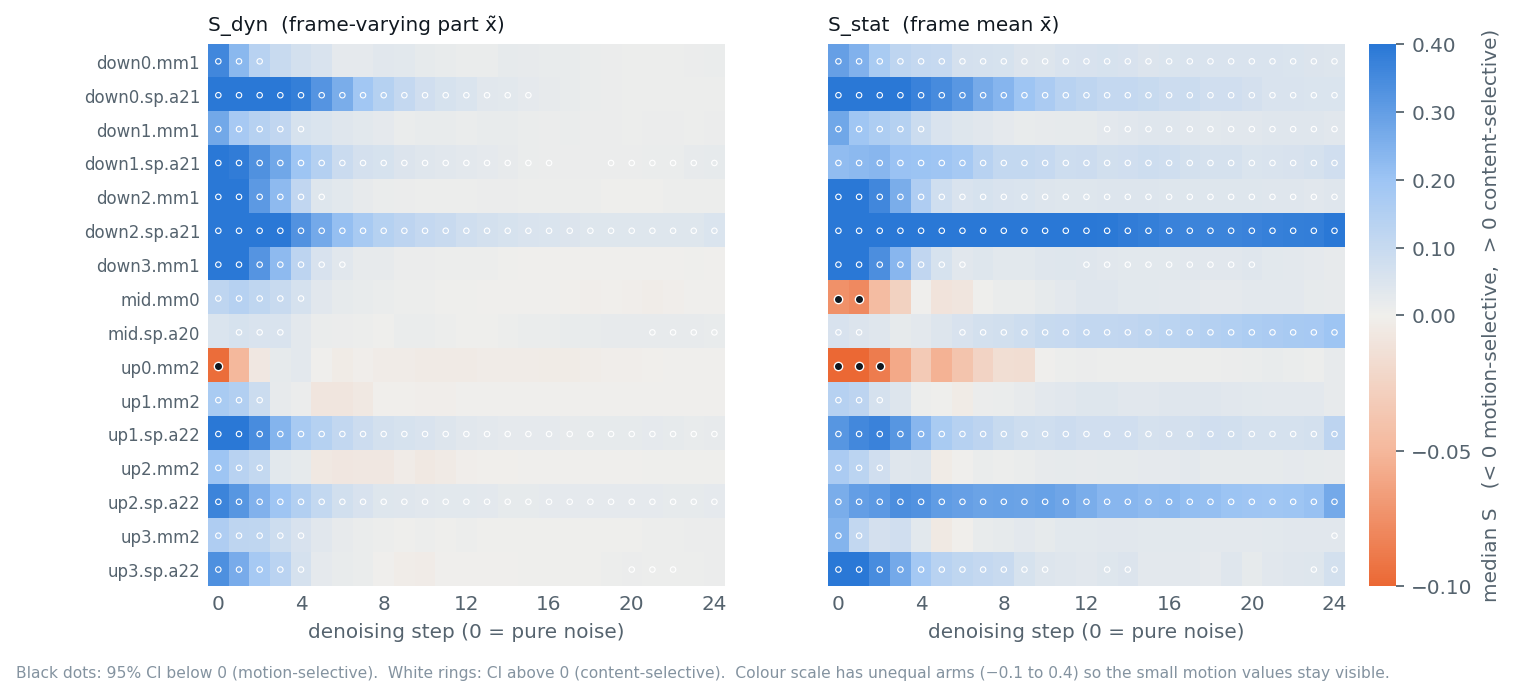
\includegraphics[width=\textwidth]{figures/sweep_selectivity_maps.png}
	\caption{Selectivity maps over 16 coordinates and 25 denoising steps (\texttt{mm} = motion module,
	\texttt{sp.a2x} = spatial cross-attention). Left: $S_{dyn}$ on the frame-varying part. Right:
	$S_{stat}$ on the frame mean. Blue is content-selective, orange motion-selective. Only
	\texttt{up0.mm2} (and \texttt{mid.mm0} in $\xs$) is motion-selective, and only in the first steps.}
	\label{fig:maps}
\end{figure}

Figure~\ref{fig:maps} is the main result of the probing stage. Almost every cell is blue: a subject swap
moves almost every layer more than a verb swap does, including the temporal layers. The spatial
cross-attention layers are the most content-selective. Every map fades towards zero after about step 9,
where content and motion swaps move the activations by similar amounts. Table~\ref{tab:hyp} gives the
three pre-registered tests.

\begin{table}[!h]
\centering
\small
\begin{tabular}{p{3.1cm}p{1.6cm}p{10.2cm}}
\toprule
Hypothesis & Verdict & Evidence \\
\midrule
H1: motion peaks at \code{up_blocks.1} & falsified & $M(b)$ is highest at \code{up_blocks.0} (+0.005), the argmax in 1000/1000 resamples. Every other block is negative: \code{up1} $-$0.017, \code{up2} $-$0.019, \code{mid} $-$0.026, \code{down0} $-$0.052, \code{down2} $-$0.075. The peak is sharp, but at the extreme (8$\times$8) resolution that the test excluded. \\
H2: motion is settled early & survives & On \code{up0.mm2}, $m(t)$ = 0.096, 0.050, 0.007, then about 0. Changepoint $\tau = 2$, 95\% CI [1, 3]; early mean 0.073 vs.\ late $-$0.001. \\
H3: removing $\xs$ reveals hidden motion & falsified & $f_{stat} = 0.65 < 0.75$ and no coordinate flips. $S_{dyn} < S_{stat}$ almost everywhere (e.g.\ \code{down2} cross-attention 0.43 $\to$ 0.17), so the split moves every coordinate towards motion, but never past zero. \\
\bottomrule
\end{tabular}
\caption{Pre-registered hypothesis tests (78 matched units per seed, 3 seeds, 1{,}000 bootstrap resamples).}
\label{tab:hyp}
\end{table}

\begin{figure}[!h]
	\centering
	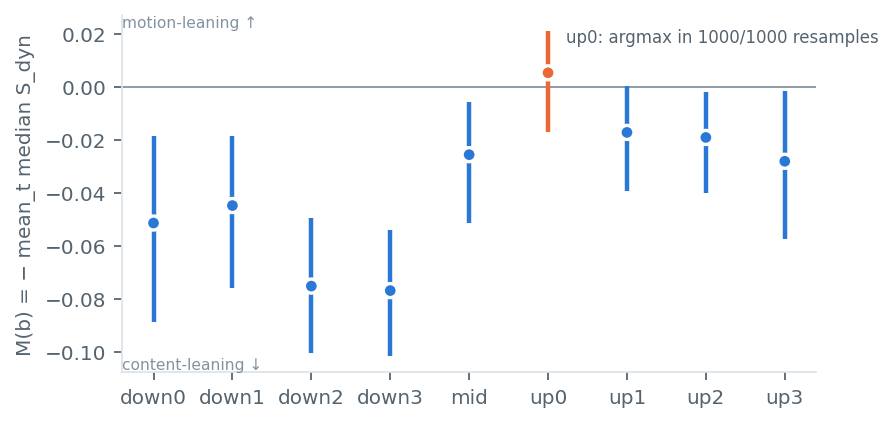
\includegraphics[width=0.49\textwidth]{figures/sweep_h1_blocks.png}\hfill
	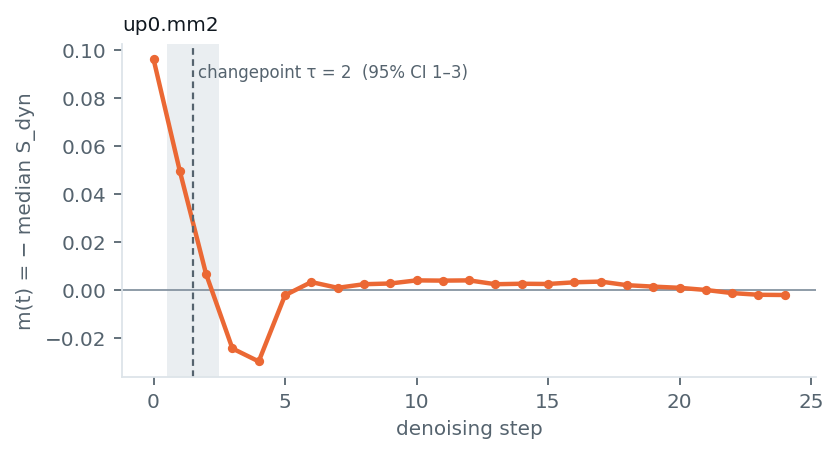
\includegraphics[width=0.49\textwidth]{figures/sweep_h2_timestep.png}
	\caption{Left: motion selectivity $M(b)$ of the nine temporal blocks with 95\% CIs; only
	\texttt{up\_blocks.0} is above zero. Right: the motion-selectivity profile of \texttt{up0.mm2} over
	the denoising steps, with the fitted changepoint and its CI.}
	\label{fig:h1h2}
\end{figure}

Two observations go beyond the tests. First, the H3 result is the opposite of what we expected: in the
very first steps the cleaner motion signal is in $\xs$, not $\xd$. $S_{stat}$ has five motion-significant
cells (\code{up0.mm2} at steps 0--2, \code{mid.mm0} at steps 0--1), while $S_{dyn}$ has only one. The static
share of the activation energy, $F\|\xs\|^2/\|x\|^2$, is 0.39--0.70 in the motion modules but 0.82--0.9996
in the spatial cross-attention layers. So ``the frame mean is content'' holds on the spatial path, not on
the temporal one. Second, on \code{up0.mm2} the motion profile dips below zero at steps 3--4 ($-$0.024,
$-$0.030) before settling. Our two-segment test was not designed to detect this, and we have not
interpreted it.

\textbf{Robustness.} Cosine and relative-L2 distances give nearly the same map (Spearman 0.987), and the
median of per-unit ratios agrees with the ratio of medians (0.930). Seed-to-seed agreement of the
$S_{dyn}$ map is only moderate (0.58, 0.69, 0.73), so cell-level detail should not be over-read.

\textbf{Linear probes.} With the scene split, the verb is decodable well above chance (0.25) in places,
for example 0.74 on the mid-block cross-attention (Figure~\ref{fig:probes}). Much of this is the verb
token leaking in through the prompt: on that coordinate the probe on $\xs$ stays at 1.0 at every step,
because cross-attention reads the text embedding directly. On the temporal modules, too, the frame mean
decodes the verb better than the residual at every step. Selectivity and decodability answer different
questions: a layer can carry the verb and still respond more to a change of subject.

\begin{figure}[!h]
	\centering
	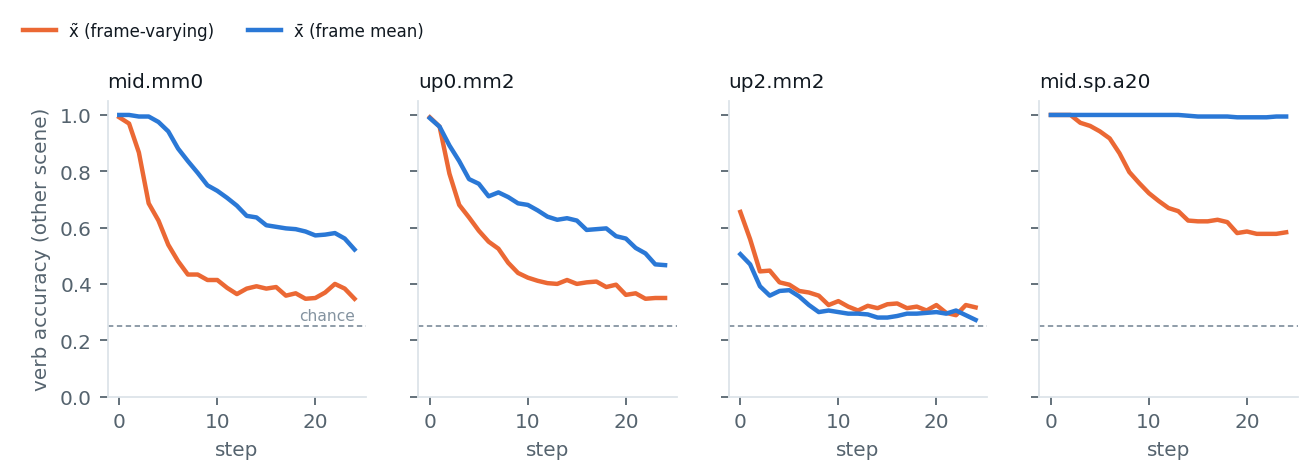
\includegraphics[width=0.8\textwidth]{figures/sweep_probes.png}
	\caption{Verb-probe accuracy over the denoising steps on four coordinates, trained on one scene and
	tested on the other (chance 0.25). $\xs$ decodes the verb at least as well as $\xd$ everywhere.}
	\label{fig:probes}
\end{figure}

\subsection{Patching controls}

\begin{table}[!h]
\centering
\small
\begin{tabular}{lll}
\toprule
Control & Result & Verdict \\
\midrule
Null patch: whole tensor, $\xd$ only, $\xs$ only, attention injection & MAD 0, PSNR $\infty$ & pass \\
Mis-indexed null patch (source from 2 steps earlier) & MAD 0.103, PSNR 25.1\,dB & detected, as required \\
Unpatched arm vs.\ the same clip as another group's source & MAD 0 & pass (no leakage) \\
Symmetry, \code{up_blocks.0}, steps 0--8: $f(A\to B)$ vs.\ $f(B\to A)$ & 0.171 vs.\ 0.083 & fail (ratio 2.06 $>$ 2) \\
\bottomrule
\end{tabular}
\caption{Controls on the real model (final run). MAD = mean absolute difference of the final latents.}
\label{tab:controls}
\end{table}

The patching machinery is exact: every null patch reproduces the unpatched clip bit for bit, and a
deliberately wrong patch is caught (Table~\ref{tab:controls}). The symmetry control fails our own
criterion. The effect has the same sign both ways, but moving the golden retriever's run into the walking
horse transfers twice as much as the reverse. One explanation is that a running clip simply has more
motion to move, but we tested only one pair, so this remains a guess.

\subsection{Edits on the held-out test pairs}

\begin{table}[!h]
\centering
\small
\begin{tabular}{llcccc}
\toprule
Direction & Arm & median $D$ & median $\dD$ & $\dD>0$ & 95\% CI \\
\midrule
keep A's motion & prompt only & 0.149 & 0 & -- & -- \\
 & $\xd$ patch, \code{up_blocks.3}, steps 0--8 (selected) & 0.195 & +0.041 & 8/12 & [$-$0.027, 0.143] \\
 & $\xd$ patch at $\alpha$ = 0.5 & 0.236 & +0.038 & 9/12 & [$-$0.031, 0.142] \\
 & whole-tensor patch, same place & 0.074 & $-$0.036 & 5/12 & [$-$0.109, 0.047] \\
 & attention injection, steps 0--8 (baseline) & 0.269 & \textbf{+0.105} & 10/12 & \textbf{[0.001, 0.204]} \\
\midrule
keep A's content & prompt only & 0.090 & 0 & -- & -- \\
 & $\xs$ patch, \code{down_blocks.3}, steps 0--8 (selected) & 0.198 & +0.068 & 10/12 & [$-$0.010, 0.158] \\
 & $\xs$ patch at $\alpha$ = 0.5 & 0.199 & +0.029 & 9/12 & [0.001, 0.152] \\
 & whole-tensor patch, same place & 0.133 & $-$0.026 & 4/12 & [$-$0.080, 0.106] \\
\bottomrule
\end{tabular}
\caption{Test-sweep results (12 pairs). $\dD$ is the paired gain over the prompt-only arm. The CI is a
95\% paired bootstrap (10{,}000 resamples) of the difference between the arm's median $D$ and the
prompt-only median $D$, which is the statistic of our success criterion, so it is not centred on the
median $\dD$. Subject consistency stayed within 1.2\% of the source for every patch arm.}
\label{tab:test}
\end{table}

Table~\ref{tab:test} answers the editing question. The pre-registered criterion is \textbf{not met}. The
selected component patches beat the prompt-only edit on the median in both directions, in 8/12 and 10/12
pairs, with subject consistency intact, but neither CI excludes zero. Three points are still clear.
\begin{itemize}
\item Component patches beat whole-tensor patches at the same site in both directions. The whole-tensor
  patch copies A wholesale. In the motion direction it reaches $s_m(\text{out},A) = 0.82$, but its content
  also moves to A ($s_c(\text{out},A) = 0.91$), so $\dD < 0$. The selected $\xd$ patch raises
  $s_m(\text{out},A)$ from 0.23 to 0.67, while $s_c(\text{out},B)$ drops only from 0.85 to 0.81. This is the
  mixing that the split was meant to remove, and it removes much of it.
\item Where motion is \emph{represented} and where patching \emph{uses} it are different places. The map
  peaks at \code{up_blocks.0}, but the best patch site in the dev sweep was the outermost, 64$\times$64
  decoder block \code{up_blocks.3}. Patching \code{up_blocks.0} gave only +0.030 there.
\item Temporal attention injection, which needs no map at all, is the strongest motion edit and the only
  motion arm whose CI excludes zero, by 0.001. In the content direction the $\xs$ patch at $\alpha = 0.5$
  also excludes zero by 0.001, but it was not the selected arm.
\end{itemize}

\textbf{Attention injection over all 25 steps.} In the dev sweep the best motion arm overall was attention
injection over the whole trajectory ($\dD$ +0.151), which the selection rule excluded because it is not a
component patch. We ran it on the test pairs in the LoRA run (E10). That run regenerated the source, B
and the prompt-only clip of every pair, and all three came out bit-identical to the test sweep's (mean
absolute latent difference 0 on all 12 pairs), so the two runs can be scored in one pool. Over all steps,
injection reaches a median $\dD$ of +0.120, positive on 11 of 12 pairs, with CI [0.020, 0.203]. It raises
$s_m(\text{out},A)$ to 0.76 while $s_c(\text{out},B)$ stays at 0.81. Adding new arms changes the min-max pool,
so the other arms move slightly (the selected $\xd$ patch +0.045, CI [$-$0.019, 0.148]; injection over
steps 0--8 +0.108, CI [0.006, 0.202]). Table~\ref{tab:test} keeps the numbers from the test run alone.
Section~\ref{sec:res_attn} shows that the same clips can fall on either side of zero in other pools.

\begin{figure}[!h]
	\centering
	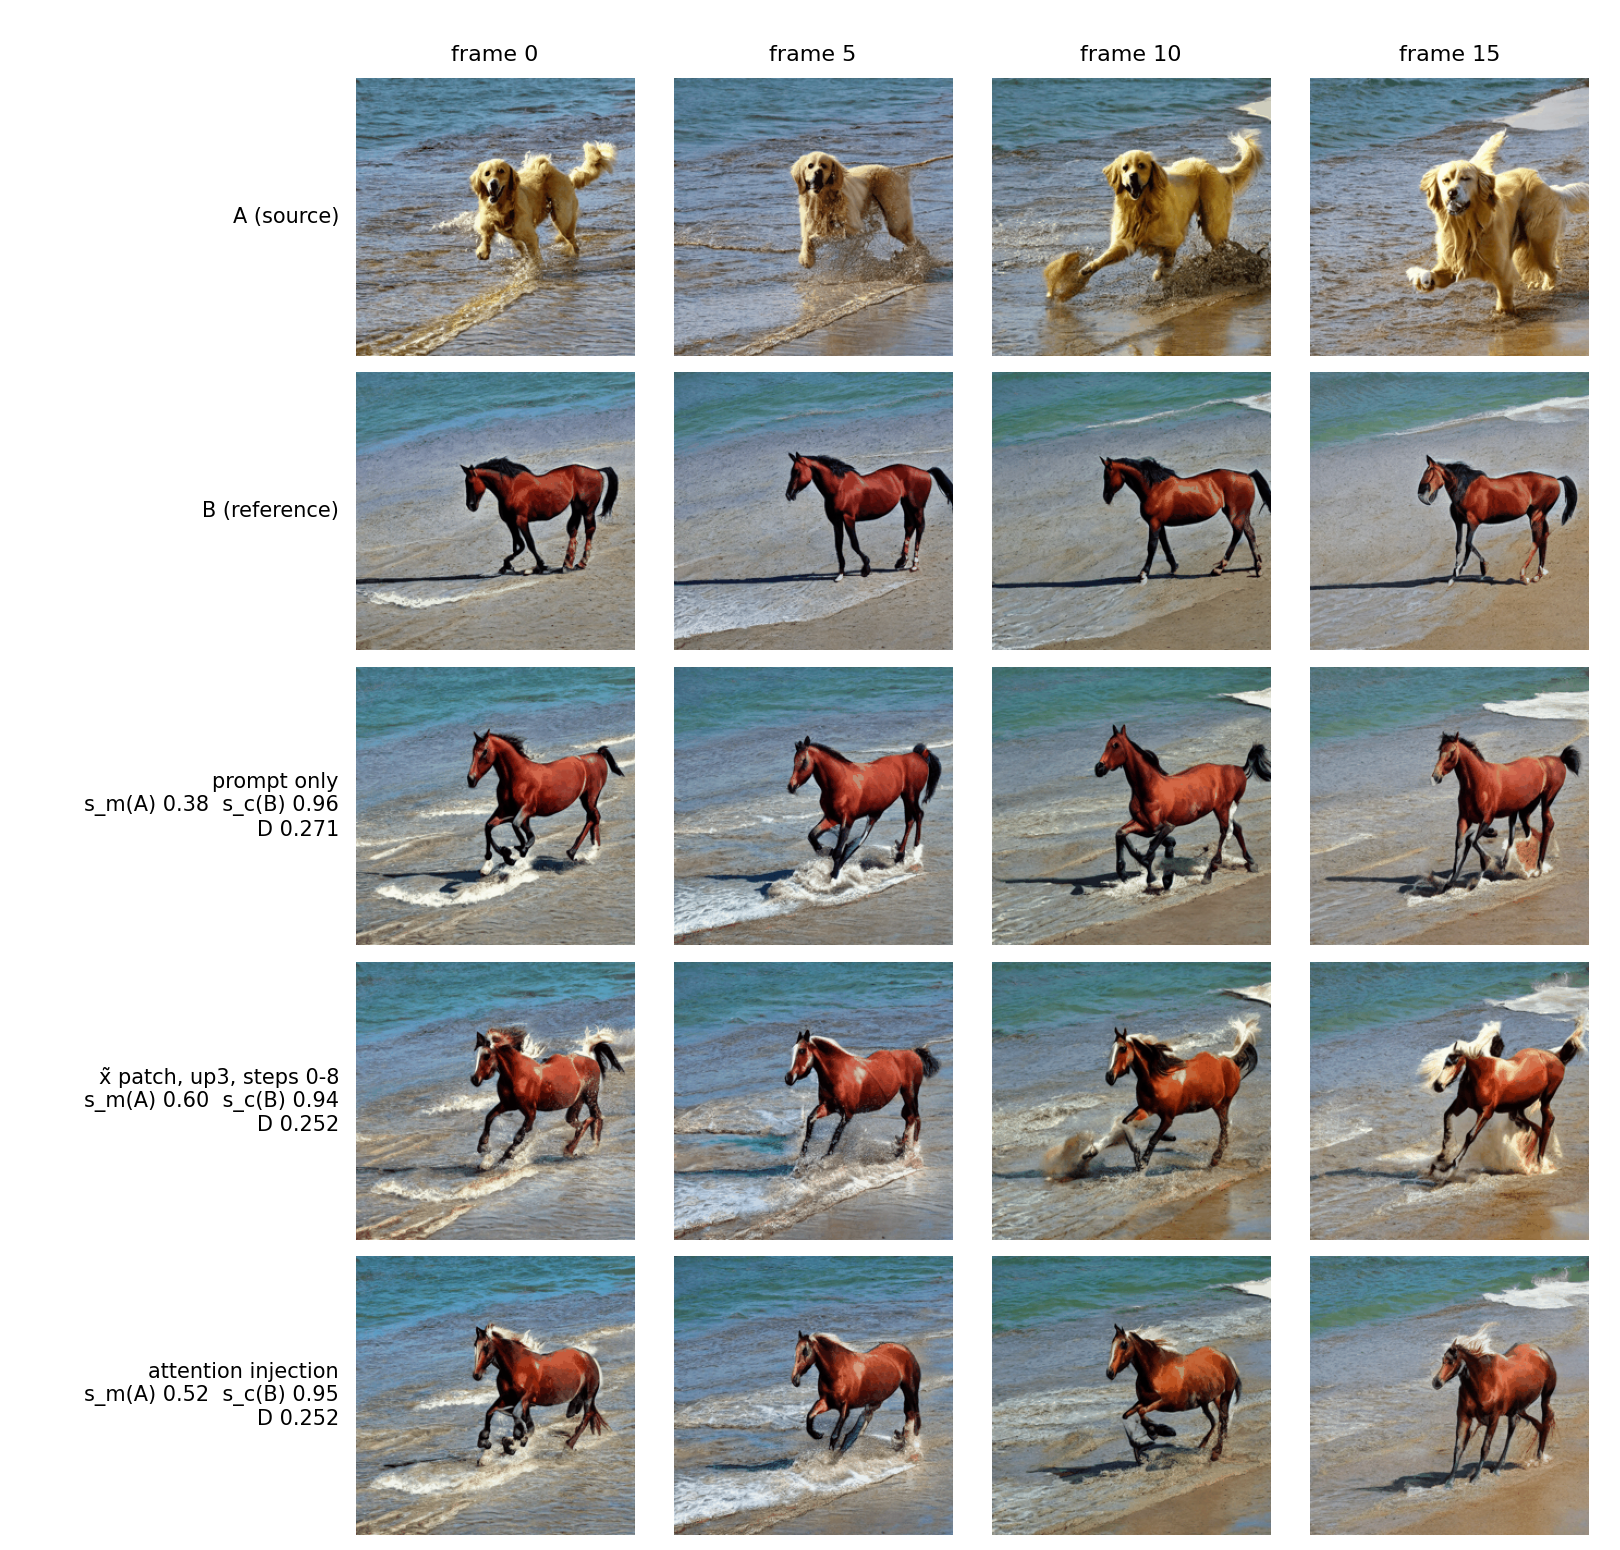
\includegraphics[width=0.86\textwidth]{figures/qual_motion_42.png}
	\caption{Motion direction on test pair 1 (``a golden retriever running'' $\to$ ``a horse walking'',
	beach, seed 42). Target prompt: ``a horse running''. The prompt-only horse runs, but in its own way.
	With the $\xd$ patch it picks up the dog's splash and stride, and its flow similarity to A rises from
	0.38 to 0.60. $D$ falls slightly on this pair because some of A's appearance comes along (the pale
	mane and spray).}
	\label{fig:qual_motion}
\end{figure}

\begin{figure}[!h]
	\centering
	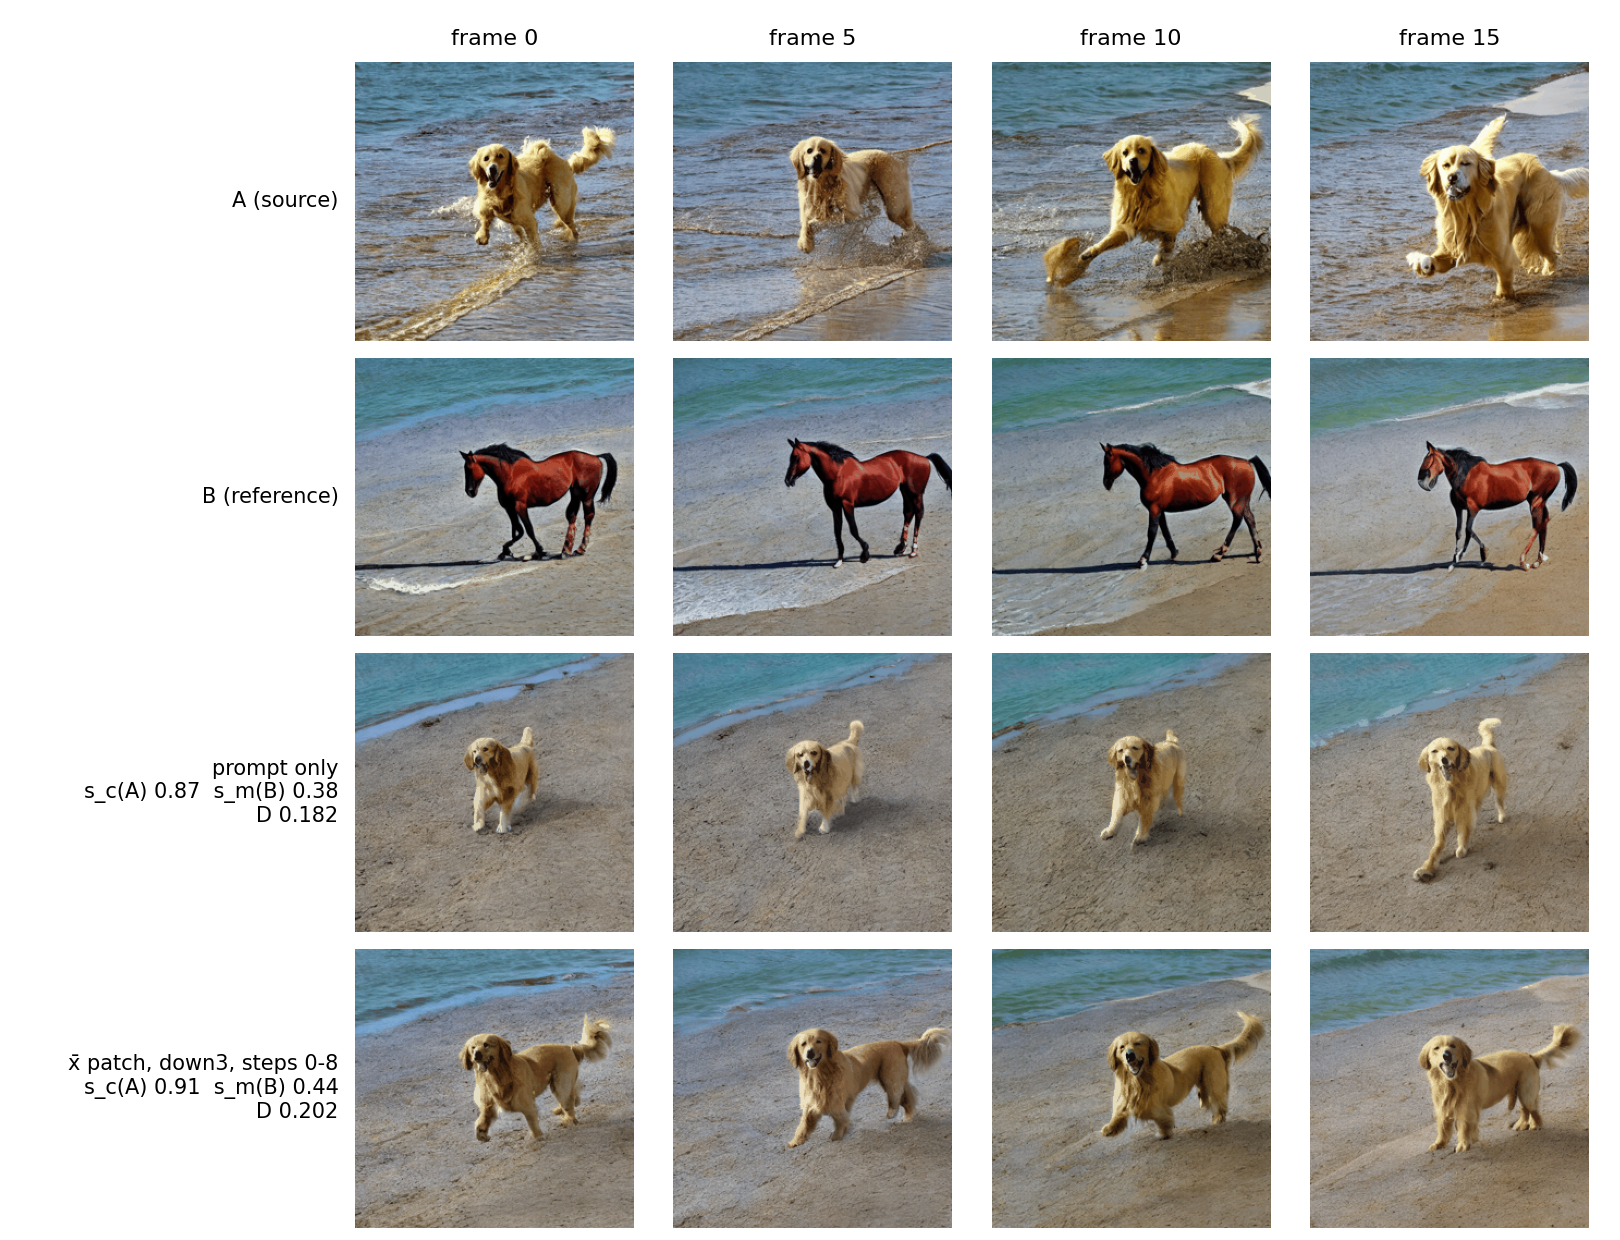
\includegraphics[width=0.86\textwidth]{figures/qual_content_42.png}
	\caption{Content direction on the same pair. Target prompt: ``a golden retriever walking''. The
	$\xs$ patch on \texttt{down\_blocks.3} keeps the source dog's build, coat and raised tail more closely
	than the prompt alone ($s_c$ to A 0.87 $\to$ 0.91) while it walks.}
	\label{fig:qual_content}
\end{figure}

Figures~\ref{fig:qual_motion} and \ref{fig:qual_content} show one pair in both directions. They also
show the limits of our metrics. CLIP similarity is a coarse measure of identity, and the flow cosine
rewards matching \emph{where} pixels move, which includes splashes and camera-like drift as well as the
animal's legs.

\subsection{Attention-level edits} \label{sec:res_attn}

\begin{table}[!h]
\centering
\small
\begin{tabular}{p{2.2cm}lp{5.6cm}ccc}
\toprule
Direction & Family & Arm & median $\dD$ & $\dD>0$ & 95\% CI \\
\midrule
keep A's motion & single & temporal attention, all modules, all steps & +0.097 & 10/12 & [$-$0.019, 0.185] \\
 & dual & + B's keys/values in \code{up_blocks.2}--\code{3} from step 2 & \textbf{+0.173} & 12/12 & \textbf{[0.111, 0.266]} \\
 & reference & attention injection, steps 0--8 & +0.096 & 9/12 & [$-$0.030, 0.213] \\
 & reference & selected $\xd$ patch & +0.028 & 8/12 & [$-$0.057, 0.123] \\
\midrule
keep A's content & single & keys/values in \code{down_blocks.2} from step 2 (probe-placed) & +0.022 & 8/12 & [$-$0.027, 0.151] \\
 & dual & A's keys/values + B's temporal attention, all steps & \textbf{+0.145} & 12/12 & \textbf{[0.102, 0.279]} \\
 & reference & selected $\xs$ patch & +0.092 & 11/12 & [0.004, 0.191] \\
\bottomrule
\end{tabular}
\caption{Attention-level edits on the 12 test pairs, all arms in one pool (exploratory). ``Reference''
arms are the earlier patches and baseline, regenerated in the same job; their clips are the same as in
Table~\ref{tab:test}, only the normalisation pool differs. Statistics as in Table~\ref{tab:test}.}
\label{tab:attn}
\end{table}

Table~\ref{tab:attn} gives the attention-level edits. The single-source arms, which edit from a prompt
like the earlier patches, do not pass our criterion. Temporal attention over all steps moves A's motion
strongly ($s_m(\text{out},A)$ 0.23 $\to$ 0.76), but A's appearance comes along with it ($s_c(\text{out},A)$
0.77 $\to$ 0.83, $s_c(\text{out},B)$ 0.85 $\to$ 0.81), and $D$ charges for that. The probe-placed key/value
arm, which was the best single content arm on the dev pairs (+0.056), adds little on test (+0.022). On the
dev pairs, the probe-placed temporal attention arms (\code{up_blocks.0} and the mid block), like
temporal attention in \code{up_blocks.0} alone, did nothing ($\dD$ between $-$0.020 and $-$0.002): injecting motion needs all temporal attention layers, not just the
place where the map peaks. This is the same gap between representation and use that we saw with the patches.

The dual-source arms pass on all 12 pairs in both directions. In the motion direction the output takes
A's motion ($s_m(\text{out},A)$ 0.23 $\to$ 0.57) with B's look ($s_c(\text{out},B)$ 0.85 $\to$ 0.89) while B's own motion
barely changes (0.17 $\to$ 0.22). In the content direction it keeps A's look ($s_c(\text{out},A)$ 0.83 $\to$ 0.90) and
takes B's motion ($s_m(\text{out},B)$ 0.26 $\to$ 0.56). As explained in Section~\ref{sec:after}, part of this
score comes from reading B directly, so this shows that we can swap motion and appearance between two
clips, not that we can edit a clip from a prompt. Looking at the clips also showed that a high $D$ on a
single pair does not guarantee a good edit: on one pair (soldier $\to$ dancer) the dual content edit scores
$D = 0.39$, but the clip shows only sand and a boot. We therefore picked the demo clips by eye.

This pool also exposes a weakness of $D$. The reference arms are the same clips as in
Table~\ref{tab:test}, but here attention injection over steps 0--8 has a CI that includes zero, and the
selected $\xs$ patch has one that excludes zero. The same happens for attention injection over all steps
(+0.097 here, +0.120 in the LoRA pool, on identical clips). Because $D$ is min-max normalised over each
run's pool, results whose CIs end within a few thousandths of zero are not stable across runs. We keep the
pre-registered verdict as it was recorded on the test run.

\subsection{Prompt switching}

\begin{figure}[!h]
	\centering
	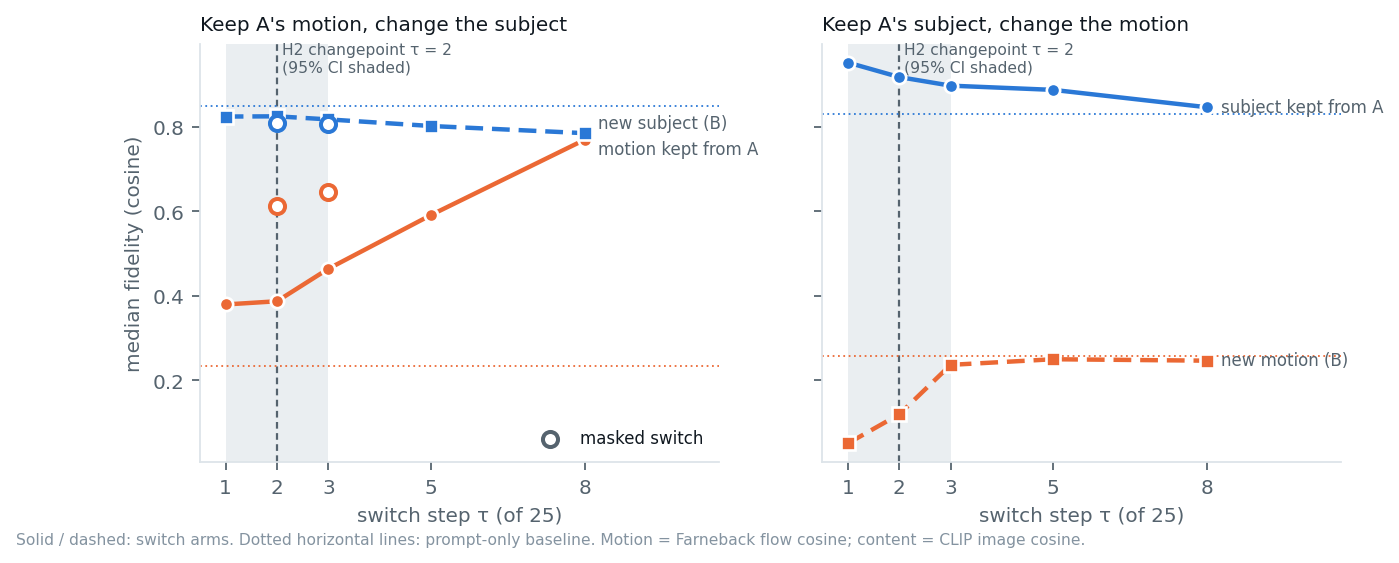
\includegraphics[width=0.9\textwidth]{figures/switch_curve.png}
	\caption{Prompt switching on the 12 test pairs, as a function of the switch step $\tau$. Left (motion
	direction): A's prompt until $\tau$, then B's subject with A's verb. Right (content direction): A's
	subject with B's verb until $\tau$, then A's prompt. Dotted lines are the prompt-only arm, and the
	shaded band is the H2 changepoint CI.}
	\label{fig:switch}
\end{figure}

None of the pre-registered $\tau = 2$ arms meets our criterion: the plain switch gives median $\dD$ +0.008
(CI [$-$0.099, 0.103]) in the motion direction and +0.016 (CI [$-$0.085, 0.144]) in the content
direction, and the masked switch +0.017 (CI [$-$0.099, 0.163]). The curves in Figure~\ref{fig:switch}
explain why, and they are a partial test of H2.
\begin{itemize}
\item In the motion direction, the motion kept from A rises steadily with $\tau$ ($s_m(\text{out},A)$ =
  0.38, 0.39, 0.46, 0.59, 0.77 at $\tau$ = 1, 2, 3, 5, 8) with no bend at $\tau = 2$. A's appearance also
  creeps in as $\tau$ grows, so $\dD$ stays near zero for every $\tau$. The masked switch raises
  $s_m(\text{out},A)$ at $\tau = 2$ from 0.39 to 0.61 with almost the same $s_c(\text{out},B)$ (0.81 vs.\
  0.83), but its gain in $D$ is not reliable. The subject masks covered 23\% to 100\% of the frame, and on
  two pairs the mask was the whole frame, so the masked switch reduced to the plain one.
\item In the content direction there is a bend. B's motion only takes hold when its prompt is kept for
  three steps: $s_m(\text{out},B)$ is 0.05 at $\tau = 1$, 0.12 at $\tau = 2$ and 0.24 at $\tau = 3$, and then
  stays at the prompt-only level (0.26). So the motion that the verb sets is fixed within the first three
  steps, which is inside the H2 CI [1, 3] but one step later than the changepoint we pre-registered.
  The exploratory arms at $\tau = 3$ (+0.065, CI [0.038, 0.086], 11/12 pairs) and $\tau = 5$ (+0.041, CI
  [0.032, 0.132], 11/12) meet the criterion. These values of $\tau$ were picked after seeing the test pairs,
  so they need new pairs before we can claim them.
\end{itemize}

\subsection{Motion LoRAs}

\begin{table}[!h]
\centering
\small
\begin{tabular}{lccccc}
\toprule
 & & \multicolumn{2}{c}{Held-out loss at step 800} & \multicolumn{2}{c}{Test pairs, prompt + LoRA, median $\dD$} \\
Variant & Params & first recipe & cut-free, seeds 0/1/2 & first recipe & cut-free, per seed \\
\midrule
untrained & -- & 0.0996 & 0.0982 & -- & -- \\
\code{full}  & 9.67\,M & 0.0638 & 0.0627 / 0.0627 / 0.0627 & $-$0.021 & +0.004 / +0.008 / $-$0.013 \\
\code{probe} & 1.97\,M & 0.0652 & 0.0641 / 0.0641 / 0.0641 & +0.023 & +0.014 / +0.015 / +0.009 \\
\code{anti}  & 2.62\,M & 0.0646 & 0.0635 / 0.0636 / 0.0635 & $-$0.020 & $-$0.011 / $-$0.031 / $-$0.001 \\
\bottomrule
\end{tabular}
\caption{Motion LoRAs. The untrained loss differs between recipes because the cut-free validation
window is the centre of the longest shot. Cut-free $\dD$ is scored in one pool with the test run
(E10). Every $\dD$ CI in the table includes zero.}
\label{tab:lora}
\end{table}

\begin{figure}[!h]
	\centering
	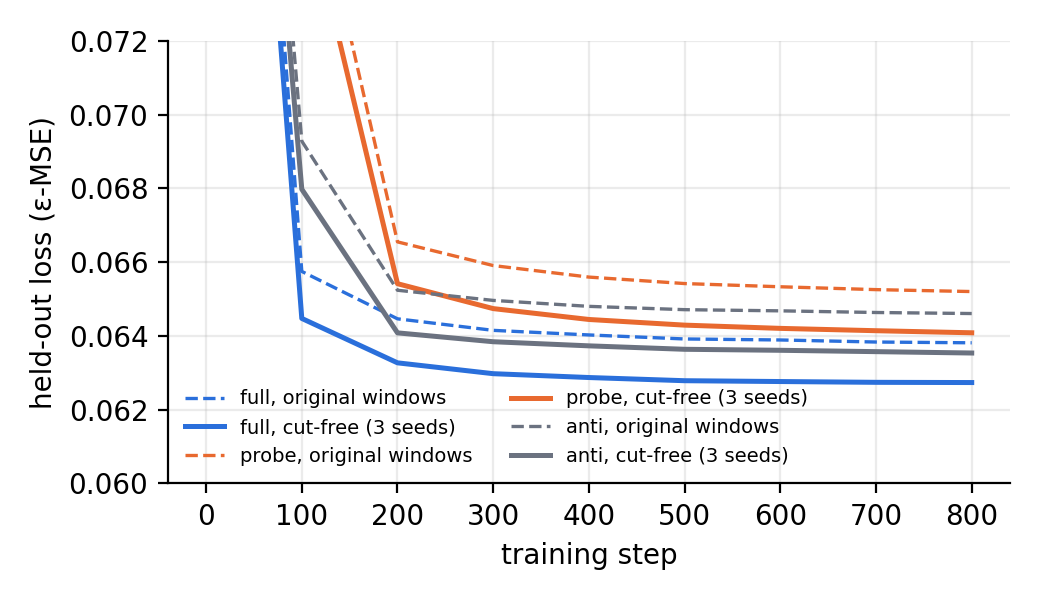
\includegraphics[width=0.62\textwidth]{figures/lora_val.png}
	\caption{Held-out loss during training. Most of the drop happens in the first 100 steps for every
	variant, which looks more like adapting to HMDB51's look (grain, low resolution) than to its motion.}
	\label{fig:lora_val}
\end{figure}

On held-out loss, size matters more than placement (Table~\ref{tab:lora}). In both recipes \code{full} is
lowest, and the wrong-place control \code{anti} ends \emph{below} the map-guided \code{probe}, with 33\%
more parameters. The ordering is the same for all three cut-free seeds, and the spread between seeds is
below $10^{-4}$, so it is not noise. The validation loss is not specific to motion, though
(Figure~\ref{fig:lora_val}). The edit test is the better measure, and there the first-recipe \code{probe}
LoRA had the only positive median $\dD$ of the three. The cut-free retrain repeats this: \code{probe} is
positive in all three seeds (+0.009 to +0.015, 6--7 of 12 pairs), while \code{full} and \code{anti} scatter
around zero. So on the edit test the map-guided placement does come out ahead, consistently but by a small
margin, and no single CI excludes zero. The raw scores qualify this gain. With \code{probe},
$s_m(\text{out},A)$ \emph{falls} from 0.23 to 0.14--0.17, while $s_m(\text{out},B)$ falls further, from 0.17 to
0.06--0.08. The LoRA makes the clip move less like B rather than more like A. That is expected: it learned
generic HMDB51 running, walking, jumping and turning, not clip A's particular motion. So we compare the
three LoRAs with one another and not with the patches.

\textbf{What the full LoRA learns, block by block.} For the \code{full} LoRA we computed the relative update
$\|\Delta W\|_F / \|W\|_F$ per temporal block and ranked the nine blocks by it, by selectivity $M(b)$, by
verb-probe accuracy on $\xd$, and by usefulness for patching (dev $\dD$). The LoRA's largest updates follow
the probe ranking (Spearman +0.83, $p = 0.005$) and peak at \code{up_blocks.0}, where both the map and the
probe peak. They do not follow patching usefulness ($-$0.27). The three low-resolution blocks have larger
relative updates in general, so part of this agreement may be due to resolution rather than motion. We have
not separated the two.

\subsection{Experiment 2: other models and causal tests} \label{sec:res_exp2}

\textbf{The Experiment 1 site does not replicate.} In all four cells the mean $S_{dyn}$ at \code{up_blocks.0}
motion module 2, steps 0--2, leans towards motion ($-$0.057, $-$0.073, $-$0.089, $-$0.095 for SD1.5 with
\mbox{v1-5-2} and \mbox{v1-5-3}, and epiCRealism with \mbox{v1-5-2} and \mbox{v1-5-3}), but the one-sided
sign-flip test does not reach $p < 0.05$ in any of them ($p$ = 0.189, 0.167, 0.063, 0.061). This includes
the primary cell, which is the same model as Experiment 1. So the direction of the Experiment 1 result
holds, but the effect is too weak to pass a test that treats subjects, not matched units, as the unit of
analysis, with two seeds instead of three.

\textbf{Exploratory maps.} After family-wise correction, no cell of any $S_{dyn}$ map is significantly
motion-selective, while 10--35 of the 1{,}075 cells are significantly content-selective. Only the two
epiCRealism cells have motion-selective cells in $S_{stat}$ (4 and 12). The variance fractions tell the
same story more directly. Averaged over the map of the primary cell, the subject explains 7.3\% of the
variance of $\xd$ and the verb 2.1\% (13.8\% and 4.0\% of $\xs$), and the verb fraction is between 2.1\% and
2.8\% in every cell. The largest named factor in $\xd$ is the seed (21--28\%), which fits the appearance
drift between seeds that we see in the clips, although we have not tested this. Once motion is measured
with flow instead of the verb, it is present almost everywhere, but weakly. The unique RSA motion share is
significant in 77--88\% of the coordinate-steps of each cell, with a median of about 0.05 and a maximum of
0.17--0.20. Flow decoding from $\xd$ beats the latent in 62--80\% of coordinate-steps, with the best gain at
0.125 and 0.138 in the SD1.5 cells (in the mid block, not at \code{up_blocks.0}) and 0.25--0.27 in the
epiCRealism cells, where the flows being decoded are very small. Keeping only the 4\% of channels most
selective for the verb (chosen on seed 42, tested on seed 1337) hardly changes $S_{dyn}$ (median 0.008 vs.\
0.006 on the primary cell), so we did not find motion concentrated in a few channels.

\textbf{What changes between models.} The layers of the four cells are similar (mean debiased CKA
0.70--0.75 between cells). Swapping the image weights changes the $S_{dyn}$ map much more than swapping the
motion adapter: 36 and 30 cells differ significantly between epiCRealism and SD1.5, all of them more
motion-leaning in epiCRealism, while only 7 and 8 cells differ between the two adapters, in both
directions. So the selectivity map depends more on the image features that enter the motion modules than
on the motion prior itself. One possible reason is that the epiCRealism clips barely move and drift less,
so their $\xd$ holds less appearance; we have not tested this.

\begin{table}[!h]
\centering
\small
\setlength{\tabcolsep}{4pt}
\begin{tabular}{p{3.6cm}cccccp{1.6cm}}
\toprule
Candidate site & E & PE (A$\to$B) & PE $-$ control & NE (B$\to$A) & other & verdict \\
\midrule
(1) \code{up0.mm2}, steps 0--2, $\xd$ (Exp.~1) & no & 0.37 [0.33, 0.42] & $-$0.02 [$-$0.05, 0.02] & 0.33 [0.25, 0.41] & 0.04 & uses (necessary) \\
(2) \code{up0.mm2} attention, steps 22--24, $\xd$ (RSA peak) & yes & 0.04 [0.02, 0.06] & $-$0.00 [$-$0.02, 0.01] & 0.06 [0.03, 0.09] & 0.00 & uses (necessary) \\
(3) \code{up_blocks.1}, 3 modules, steps 0--7, $\xd$ & yes & 0.74 [0.70, 0.78] & 0.17 [0.12, 0.22] & 0.69 [0.63, 0.75] & 0.17 & uses (both) \\
(4) mid-block self-attention, steps 0--3, $\xs$ (content) & yes & 0.05 [$-$0.03, 0.15] & 0.10 [0.00, 0.21] & $-$0.01 [$-$0.04, 0.01] & 0.29 & encodes, not used \\
\bottomrule
\end{tabular}
\caption{Causal tests on the primary cell (25 motion and 25 content pairs from the held-out seed, 95\% CIs
from a bootstrap over subjects). PE and NE are measured on the site's own property (motion for 1--3,
content for 4). ``Other'' is the transfer of the other property under A$\to$B, which must stay
within $\pm 0.1$ for dissociation.}
\label{tab:exp2}
\end{table}

\textbf{Causal tests.} Table~\ref{tab:exp2} gives the four candidate sites. The Experiment 1 site moves
motion when patched from A (PE 0.37), but no more than patching from an unrelated clip does, so the
sufficiency test fails: the effect looks like general disruption rather than A's motion in particular. It is necessary, though: putting
B's activation into A moves A's motion a third of the way towards B's (NE 0.33). The RSA motion peak, at the very end of
the trajectory, has the largest unique motion share but almost no causal effect (0.04 to 0.06). The
\code{up_blocks.1} motion modules, the site from the literature, are the only one that is both
sufficient and necessary, and by a wide margin, but patching them also moves content (0.17), so they fail
the dissociation test. The content site carries content (E holds) but patching it moves motion (0.29) more
than content, so it ``encodes but does not use'' content. LEACE erasure of the verb at sites (1) and (2)
did not hurt motion more than a random erasure of the same rank (differences 0.008, CI [$-$0.025, 0.037],
and 0.000, CI [$-$0.014, 0.011]). No pair of sites shows a double dissociation, so by our own rule we
cannot name \emph{the} motion site of this model.

\subsection{Upload path} \label{sec:res_upload}

\begin{table}[!h]
\centering
\small
\begin{tabular}{lcccc}
\toprule
New clip starts from & prompt only & selected $\xd$ patch & attention, steps 0--8 & attention, all steps \\
\midrule
inverted noise & 0.118 & 0.519 (hybrid, artefacts) & 0.309 & \textbf{0.668} \\
blend of inverted and Gaussian & 0.322 & 0.025 (diverges) & 0.395 & \textbf{0.656} \\
Gaussian noise & 0.085 & 0.087 (diverges) & $-$0.053 & 0.366 \\
\bottomrule
\end{tabular}
\caption{Uploaded video (a baseball pitch) turned into ``a tiger jumping'': flow cosine of the new clip
to the upload. CLIP match to the target prompt is 0.33--0.36 for every clip that did not diverge.}
\label{tab:upload}
\end{table}

The component patch does not survive this setting (Table~\ref{tab:upload}). Logging norms inside the
patcher showed why. For a generated pair the frame-varying parts of source and target already agree
closely, since both start from the same noise, so the patch is a small nudge. For an uploaded video they
are unrelated: the difference at \code{up_blocks.3} is up to 12{,}400 against an output norm of 8--21
thousand at step 0, the target's norm grows every step, and the final latent has a standard deviation of
26 instead of 0.7. The patch is a tool for pairs that share their initial noise, not a general motion
transplant. The interface therefore defaults to attention injection over all steps from the blended start
for uploads. A second clip exposed another limit: a woman walking towards the camera became a scene that
grows towards the camera, while the robot in it stayed small and nearly still. Temporal attention carries
\emph{where} things move in the frame, not \emph{which object} moves.

\subsection{Interface}

We checked all four tabs through the running app, using the same handlers as the buttons. A live edit (4
clips) takes 4.5--7 minutes on the laptop GPU at 6.4\,GB peak memory, an upload edit about 4.5 minutes,
and the results browser and the maps need no GPU. The attention-level edits were also checked live on a
T4. Invalid combinations, such as attention injection in the content direction, are rejected with a
message rather than an error.

\section{Plan for Novelty Assessment} \label{sec:Plan for Novelty Assessment}

The results leave four open questions, and the plan follows them.
\begin{enumerate}
\item \textbf{Is the split an artefact of AnimateDiff's training recipe?} Experiment 2 varied the image
  and motion weights, but all four cells are still AnimateDiff on SD1.5. We will run the same sweep (same
  vocabulary, same tests) on a model trained jointly on space and time, such as ModelScope T2V or
  VideoCrafter2. If the results come out the same, the map describes video diffusion more generally; if
  not, it describes AnimateDiff.
\item \textbf{Combine what each method is good at.} Attention injection transfers \emph{where} things move,
  and the $\xd$ patch carries \emph{which} motion at the cost of some appearance. Attention injection with a
  mask from the subject's cross-attention, so that motion lands on the object, is the most direct fix for
  the failure in the upload path. Our masked prompt switch is a first step in this direction, and the
  masked injection can be tested on the same pairs.
\item \textbf{Statistical power.} The causal tests of Experiment 2 already use 25 pairs per claim. For the
  edits we will add a second set of 24 pairs drawn by the same rule, report both sets, confirm the
  $\tau = 3$ prompt switch on them, and run the symmetry control on all pairs instead of one.
\item \textbf{Better measurements and the unfinished parts.} Replace the optical-flow cosine with point
  tracks (CoTracker \citep{karaev2024cotracker}) and CLIP with DINO features for identity, fix one pool for
  normalising $D$, and separate the resolution effect in the LoRA update ranking by normalising per
  resolution level. We will also finish the content ladder and run the LoRA test against random module sets.
\end{enumerate}

\section{Conclusion} \label{sec:conclusion}

We asked where a video diffusion U-Net keeps content and where it keeps motion, using AnimateDiff and a
controlled set of 750 one-word-swap pairs generated from shared noise. The answer is narrower than the
architecture suggests. Content dominates almost every layer, temporal ones included. Motion is selective
in only one place, the motion module just after the bottleneck, and only during the first two or three of
25 denoising steps. Removing the frame mean shifts every layer towards motion but reveals no hidden motion
layer, and two of our three pre-registered hypotheses were falsified. When we repeated the probing on four
model variants, the motion site kept its direction but did not pass a subject-level test, and motion
measured with optical flow turned out to be weakly present almost everywhere rather than concentrated in
one place.

Turning the static/dynamic split into a patch gives edits that beat changing the prompt and beat
whole-tensor patching in both directions, but not by a margin that 12 test pairs can confirm. Temporal
attention injection did better, and two-clip attention edits passed our criterion, though they read the
clip they are scored against. Switching the prompt showed that the motion set by the verb is fixed within
the first three steps. Across all of these, the place where the map says motion is represented is not
where intervening works best. The causal tests make this concrete: the Experiment 1 site is necessary for
motion but not sufficient, and the \code{up_blocks.1} motion modules from the literature are both, but move
content too. A LoRA placed by the map was not better on held-out loss than one placed where the map says
motion is absent, but it was the only placement that improved the edit in all three seeds, by a small
margin. Our measurements are exact (null patches are bit-identical) and every decision was fixed before
the data it affected, so the negative results are results too. All code, the LoRAs and an interface for
trying the edits are released with this report.


\begin{thebibliography}{99}
\setlength{\itemsep}{1pt}
\small

\bibitem{baherwani2025timesteps} Vatsal Baherwani, Yixuan Ren, and Abhinav Shrivastava. Characterizing motion encoding in video diffusion timesteps, arXiv preprint, 2025. \url{https://arxiv.org/abs/2512.22175}

\bibitem{bai2024uniedit} Jianhong Bai, Tianyu He, Yuchi Wang, Junliang Guo, Haoji Hu, Zuozhu Liu, and Jiang Bian. UniEdit: A unified tuning-free framework for video motion and appearance editing, arXiv preprint, 2024. \url{https://arxiv.org/abs/2402.13185}

\bibitem{basu2024localizing} Samyadeep Basu, Nanxuan Zhao, Vlad Morariu, Soheil Feizi, and Varun Manjunatha. Localizing and editing knowledge in text-to-image generative models, International Conference on Learning Representations (ICLR), 2024. \url{https://arxiv.org/abs/2310.13730}

\bibitem{belrose2023leace} Nora Belrose, David Schneider-Joseph, Shauli Ravfogel, Ryan Cotterell, Edward Raff, and Stella Biderman. LEACE: Perfect linear concept erasure in closed form, Advances in Neural Information Processing Systems (NeurIPS), 2023. \url{https://arxiv.org/abs/2306.03819}

\bibitem{blattmann2023align} Andreas Blattmann, Robin Rombach, Huan Ling, Tim Dockhorn, Seung Wook Kim, Sanja Fidler, and Karsten Kreis. Align your latents: High-resolution video synthesis with latent diffusion models, IEEE/CVF Conference on Computer Vision and Pattern Recognition (CVPR), 2023. \url{https://arxiv.org/abs/2304.08818}

\bibitem{cao2023masactrl} Mingdeng Cao, Xintao Wang, Zhongang Qi, Ying Shan, Xiaohu Qie, and Yinqiang Zheng. MasaCtrl: Tuning-free mutual self-attention control for consistent image synthesis and editing, IEEE/CVF International Conference on Computer Vision (ICCV), 2023. \url{https://arxiv.org/abs/2304.08465}

\bibitem{caron2021dino} Mathilde Caron, Hugo Touvron, Ishan Misra, Herv\'e J\'egou, Julien Mairal, Piotr Bojanowski, and Armand Joulin. Emerging properties in self-supervised vision transformers, IEEE/CVF International Conference on Computer Vision (ICCV), 2021. \url{https://arxiv.org/abs/2104.14294}

\bibitem{elazar2021amnesic} Yanai Elazar, Shauli Ravfogel, Alon Jacovi, and Yoav Goldberg. Amnesic probing: Behavioral explanation with amnesic counterfactuals, Transactions of the Association for Computational Linguistics (TACL), 2021. \url{https://aclanthology.org/2021.tacl-1.10/}

\bibitem{farneback2003} Gunnar Farneb\"ack. Two-frame motion estimation based on polynomial expansion, Scandinavian Conference on Image Analysis (SCIA), 2003. \url{https://doi.org/10.1007/3-540-45103-X_50}

\bibitem{guo2024animatediff} Yuwei Guo, Ceyuan Yang, Anyi Rao, Zhengyang Liang, Yaohui Wang, Yu Qiao, Maneesh Agrawala, Dahua Lin, and Bo Dai. AnimateDiff: Animate your personalized text-to-image diffusion models without specific tuning, International Conference on Learning Representations (ICLR), 2024. \url{https://arxiv.org/abs/2307.04725}

\bibitem{heimersheim2024patching} Stefan Heimersheim and Neel Nanda. How to use and interpret activation patching, arXiv preprint, 2024. \url{https://arxiv.org/abs/2404.15255}

\bibitem{hertz2023p2p} Amir Hertz, Ron Mokady, Jay Tenenbaum, Kfir Aberman, Yael Pritch, and Daniel Cohen-Or. Prompt-to-prompt image editing with cross attention control, International Conference on Learning Representations (ICLR), 2023. \url{https://arxiv.org/abs/2208.01626}

\bibitem{hewitt2019control} John Hewitt and Percy Liang. Designing and interpreting probes with control tasks, Conference on Empirical Methods in Natural Language Processing (EMNLP), 2019. \url{https://arxiv.org/abs/1909.03368}

\bibitem{ho2020ddpm} Jonathan Ho, Ajay Jain, and Pieter Abbeel. Denoising diffusion probabilistic models, Advances in Neural Information Processing Systems (NeurIPS), 2020. \url{https://arxiv.org/abs/2006.11239}

\bibitem{ho2021cfg} Jonathan Ho and Tim Salimans. Classifier-free diffusion guidance, NeurIPS Workshop on Deep Generative Models and Downstream Applications, 2021. \url{https://arxiv.org/abs/2207.12598}

\bibitem{ho2022vdm} Jonathan Ho, Tim Salimans, Alexey Gritsenko, William Chan, Mohammad Norouzi, and David J. Fleet. Video diffusion models, Advances in Neural Information Processing Systems (NeurIPS), 2022. \url{https://arxiv.org/abs/2204.03458}

\bibitem{hu2022lora} Edward J. Hu, Yelong Shen, Phillip Wallis, Zeyuan Allen-Zhu, Yuanzhi Li, Shean Wang, Lu Wang, and Weizhu Chen. LoRA: Low-rank adaptation of large language models, International Conference on Learning Representations (ICLR), 2022. \url{https://arxiv.org/abs/2106.09685}

\bibitem{huang2024vbench} Ziqi Huang, Yinan He, Jiashuo Yu, Fan Zhang, Chenyang Si, Yuming Jiang, Yuanhan Zhang, Tianxing Wu, Qingyang Jin, Nattapol Chanpaisit, Yaohui Wang, Xinyuan Chen, Limin Wang, Dahua Lin, Yu Qiao, and Ziwei Liu. VBench: Comprehensive benchmark suite for video generative models, IEEE/CVF Conference on Computer Vision and Pattern Recognition (CVPR), 2024. \url{https://arxiv.org/abs/2311.17982}

\bibitem{jagpal2025eidtv} Diljeet Jagpal, Xi Chen, and Vinay P. Namboodiri. EIDT-V: Exploiting intersections in diffusion trajectories for model-agnostic, zero-shot, training-free text-to-video generation, IEEE/CVF Conference on Computer Vision and Pattern Recognition (CVPR), 2025. \url{https://arxiv.org/abs/2504.06861}

\bibitem{karaev2024cotracker} Nikita Karaev, Ignacio Rocco, Benjamin Graham, Natalia Neverova, Andrea Vedaldi, and Christian Rupprecht. CoTracker: It is better to track together, European Conference on Computer Vision (ECCV), 2024. \url{https://arxiv.org/abs/2307.07635}

\bibitem{kornblith2019cka} Simon Kornblith, Mohammad Norouzi, Honglak Lee, and Geoffrey Hinton. Similarity of neural network representations revisited, International Conference on Machine Learning (ICML), 2019. \url{https://arxiv.org/abs/1905.00414}

\bibitem{kriegeskorte2008rsa} Nikolaus Kriegeskorte, Marieke Mur, and Peter Bandettini. Representational similarity analysis: connecting the branches of systems neuroscience, Frontiers in Systems Neuroscience, 2008. \url{https://doi.org/10.3389/neuro.06.004.2008}

\bibitem{kuehne2011hmdb} Hildegard Kuehne, Hueihan Jhuang, Est\'ibaliz Garrote, Tomaso Poggio, and Thomas Serre. HMDB: A large video database for human motion recognition, IEEE International Conference on Computer Vision (ICCV), 2011. \url{https://doi.org/10.1109/ICCV.2011.6126543}

\bibitem{ling2025motionclone} Pengyang Ling, Jiazi Bu, Pan Zhang, Xiaoyi Dong, Yuhang Zang, Tong Wu, Huaian Chen, Jiaqi Wang, and Yi Jin. MotionClone: Training-free motion cloning for controllable video generation, International Conference on Learning Representations (ICLR), 2025. \url{https://arxiv.org/abs/2406.05338}

\bibitem{meng2022rome} Kevin Meng, David Bau, Alex Andonian, and Yonatan Belinkov. Locating and editing factual associations in GPT, Advances in Neural Information Processing Systems (NeurIPS), 2022. \url{https://arxiv.org/abs/2202.05262}

\bibitem{ni2022xclip} Bolin Ni, Houwen Peng, Minghao Chen, Songyang Zhang, Gaofeng Meng, Jianlong Fu, Shiming Xiang, and Haibin Ling. Expanding language-image pretrained models for general video recognition, European Conference on Computer Vision (ECCV), 2022. \url{https://arxiv.org/abs/2208.02816}

\bibitem{radford2021clip} Alec Radford, Jong Wook Kim, Chris Hallacy, Aditya Ramesh, Gabriel Goh, Sandhini Agarwal, Girish Sastry, Amanda Askell, Pamela Mishkin, Jack Clark, Gretchen Krueger, and Ilya Sutskever. Learning transferable visual models from natural language supervision, International Conference on Machine Learning (ICML), 2021. \url{https://arxiv.org/abs/2103.00020}

\bibitem{rombach2022ldm} Robin Rombach, Andreas Blattmann, Dominik Lorenz, Patrick Esser, and Bj\"orn Ommer. High-resolution image synthesis with latent diffusion models, IEEE/CVF Conference on Computer Vision and Pattern Recognition (CVPR), 2022. \url{https://arxiv.org/abs/2112.10752}

\bibitem{ronneberger2015unet} Olaf Ronneberger, Philipp Fischer, and Thomas Brox. U-Net: Convolutional networks for biomedical image segmentation, International Conference on Medical Image Computing and Computer-Assisted Intervention (MICCAI), 2015. \url{https://arxiv.org/abs/1505.04597}

\bibitem{song2021ddim} Jiaming Song, Chenlin Meng, and Stefano Ermon. Denoising diffusion implicit models, International Conference on Learning Representations (ICLR), 2021. \url{https://arxiv.org/abs/2010.02502}

\bibitem{tang2023daam} Raphael Tang, Linqing Liu, Akshat Pandey, Zhiying Jiang, Gefei Yang, Karun Kumar, Pontus Stenetorp, Jimmy Lin, and Ferhan Ture. What the DAAM: Interpreting Stable Diffusion using cross attention, Annual Meeting of the Association for Computational Linguistics (ACL), 2023. \url{https://aclanthology.org/2023.acl-long.310/}

\bibitem{teed2020raft} Zachary Teed and Jia Deng. RAFT: Recurrent all-pairs field transforms for optical flow, European Conference on Computer Vision (ECCV), 2020. \url{https://arxiv.org/abs/2003.12039}

\bibitem{voita2020mdl} Elena Voita and Ivan Titov. Information-theoretic probing with minimum description length, Conference on Empirical Methods in Natural Language Processing (EMNLP), 2020. \url{https://arxiv.org/abs/2003.12298}

\bibitem{wu2023tav} Jay Zhangjie Wu, Yixiao Ge, Xintao Wang, Stan Weixian Lei, Yuchao Gu, Yufei Shi, Wynne Hsu, Ying Shan, Xiaohu Qie, and Mike Zheng Shou. Tune-A-Video: One-shot tuning of image diffusion models for text-to-video generation, IEEE/CVF International Conference on Computer Vision (ICCV), 2023. \url{https://arxiv.org/abs/2212.11565}

\bibitem{xiao2024moft} Zeqi Xiao, Yifan Zhou, Shuai Yang, and Xingang Pan. Video diffusion models are training-free motion interpreter and controller, Advances in Neural Information Processing Systems (NeurIPS), 2024. \url{https://arxiv.org/abs/2405.14864}

\bibitem{yatim2024dmt} Danah Yatim, Rafail Fridman, Omer Bar-Tal, Yoni Kasten, and Tali Dekel. Space-time diffusion features for zero-shot text-driven motion transfer, IEEE/CVF Conference on Computer Vision and Pattern Recognition (CVPR), 2024. \url{https://arxiv.org/abs/2311.17009}

\bibitem{zhang2024patching} Fred Zhang and Neel Nanda. Towards best practices of activation patching in language models: Metrics and methods, International Conference on Learning Representations (ICLR), 2024. \url{https://arxiv.org/abs/2309.16042}

\bibitem{zhao2024motiondirector} Rui Zhao, Yuchao Gu, Jay Zhangjie Wu, David Junhao Zhang, Jiawei Liu, Weijia Wu, Jussi Keppo, and Mike Zheng Shou. MotionDirector: Motion customization of text-to-video diffusion models, European Conference on Computer Vision (ECCV), 2024. \url{https://arxiv.org/abs/2310.08465}

\bibitem{hf_animatediff} Yuwei Guo and others. \url{https://huggingface.co/guoyww/animatediff-motion-adapter-v1-5-2}, Accessed on: 20th October, 2026.

\bibitem{hf_animatediff_v3} Yuwei Guo and others. \url{https://huggingface.co/guoyww/animatediff-motion-adapter-v1-5-3}, Accessed on: 26th October, 2026.

\bibitem{hf_epicrealism} emilianJR. \url{https://huggingface.co/emilianJR/epiCRealism}, Accessed on: 26th October, 2026.

\bibitem{hf_diffusers} Hugging Face. \url{https://huggingface.co/docs/diffusers}, Accessed on: 20th October, 2026.

\bibitem{hf_hmdb} DIVM. \url{https://huggingface.co/datasets/divm/hmdb51}, Accessed on: 20th October, 2026.

\end{thebibliography}

\end{document}
